\documentclass[]{beamer}
% Class options include: notes, notesonly, handout, trans,
%                        hidesubsections, shadesubsections,
%                        inrow, blue, red, grey, brown

% Theme for beamer presentation.
\usepackage{beamerthemesplit} 
\usepackage{multimedia}
\usepackage{hyperref}

\usepackage{collectbox}

\usepackage[utf8]{inputenc}
\usepackage[english]{babel}

%%%%%%%%%%%%%%%%%%%%%%%%%%%%%%%%%%%%%%%%%%%%%%%%%%%%%%%%%%%%%%%%%%%%%%



\definecolor{mypink1}{rgb}{0.858, 0.188, 0.478}

\newcommand{\mybox}{%
    \collectbox{%
        \setlength{\fboxsep}{1pt}%
        \fbox{\BOXCONTENT}%
    }%
}

%%%%%%%%%%%%%%%%%%%%%%%%%%%%%%%%%%%%%%%%%%%%%%%%%%%%%%%%%%%%%%%%%%%%%%
% Other themes include: beamerthemebars, beamerthemelined, 
%                       beamerthemetree, beamerthemetreebars  

\title{PHY250: FLUIDS IN MOTION}    % Enter your title between curly braces
\author{Anabela R. Turlione}                 % Enter your name between curly braces
\institute{Digipen}      % Enter your institute name between curly braces
\date{Fall 2021}                    % Enter the date or \today between curly braces


\begin{document}

% Creates title page of slide show using above information
\begin{frame}
  \titlepage
\end{frame}
%\note{Talk for 30 minutes} % Add notes to yourself that will be displayed when
                           % typeset with the notes or notesonly class options

\section[]{}

% Creates table of contents slide incorporating
% all \section and \subsection commands
\begin{frame}
  \tableofcontents
\end{frame}


% \begin{frame}
%   % \centering
%    \movie[externalviewer]{\includegraphics[width=\textheight ,
%    keepaspectratio]{surfacet1.jpg}}{test.mp4}

% \end{frame}
%%%%%%%%%%%%%%%%%%%%%%%%%%%%%%%%%%%%%%%%%%%%%%%%%%%%%%%%%%%%%%%%%%%




\section{Fluids Dynamic}

\begin{frame}
  \frametitle{Fluids in motion}


In general, the equation $\nabla P+\rho \nabla \phi =0$  has no solution.
\vspace{5mm}
\pause


\begin{center}
  $\rightarrow$ $\nabla P+\rho \nabla \phi =\rho \vec{a}$

\vspace{10mm}

  \textcolor{mypink1}{  \boxed{Dynamic~Fluid}}
\end{center}

  \end{frame}

%%%%%%%%%%%%%%%%%%%%%%%%%%%%%%%%%%%%%%%%%%%%%%%%%%%%%%%%%%%%%%%



\begin{frame}
  \frametitle{Fluids in motion}
To describe the motion of a fluid, we need:


\vspace{5 mm}

\pause
\begin{itemize}
  \item An equation of state: $P(\rho)$
  \item The velocity at every point
\end{itemize}



  \end{frame}

  %%%%%%%%%%%%%%%%%%%%%%%%%%%%%%%%%%%%%%%%%%%%%%%%%%%%%%%%%%%%%%%



\begin{frame}


  \begin{center}
    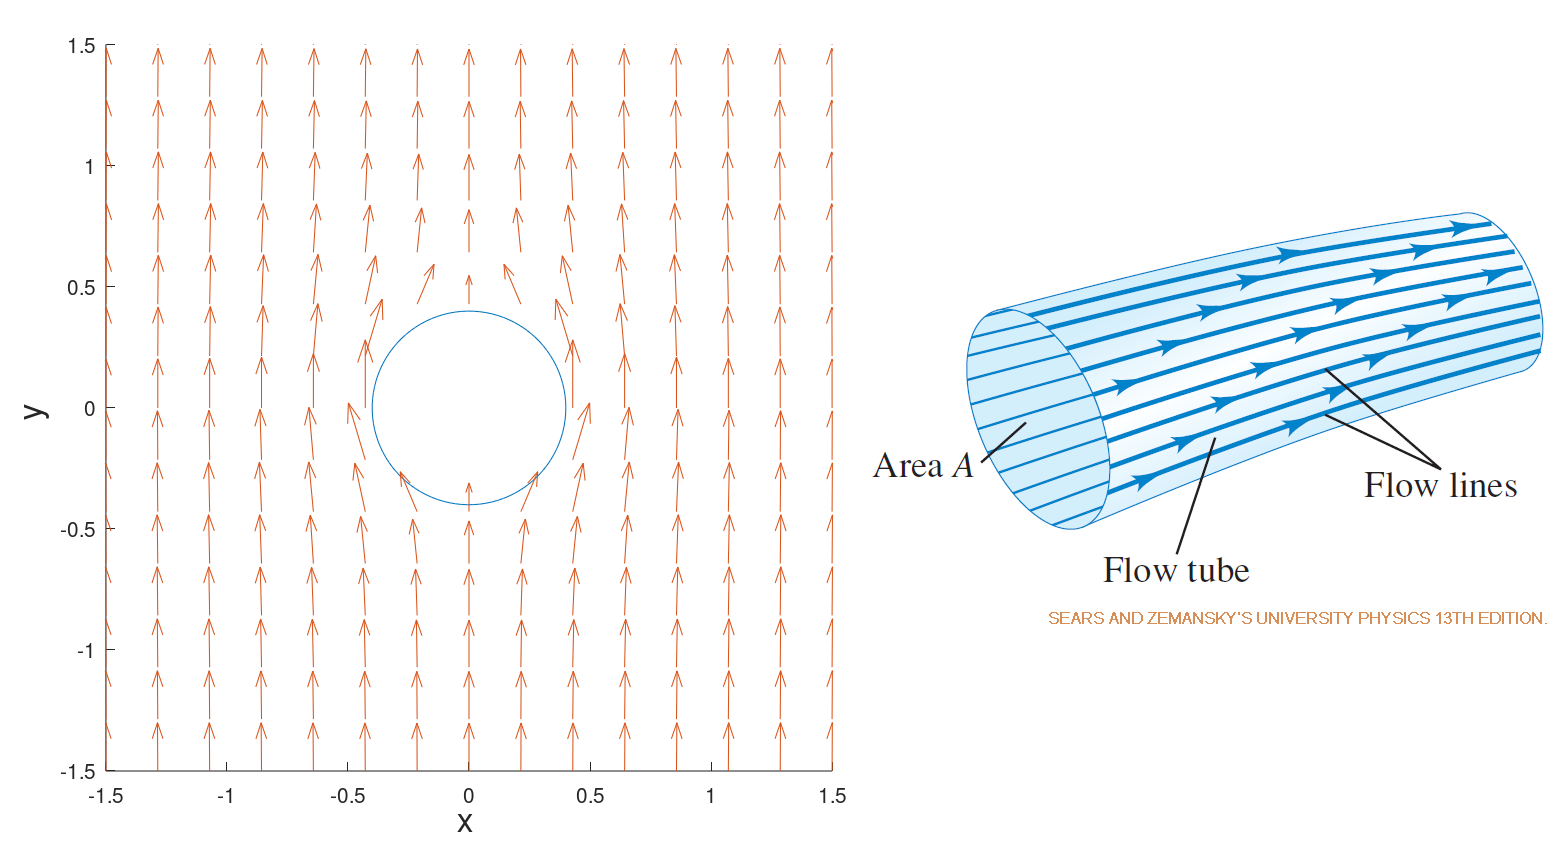
\includegraphics[height=2.5in]{images2/Vector_field_v.png}
  \end{center}

  

  \end{frame}

  %%%%%%%%%%%%%%%%%%%%%%%%%%%%%%%%%%%%%%%%%%%%%%%%%%%%%%%%%%%%%%%

  \begin{frame}

 Streamlines: lines which are always tangent to the fluid velocity.

 \begin{center}
  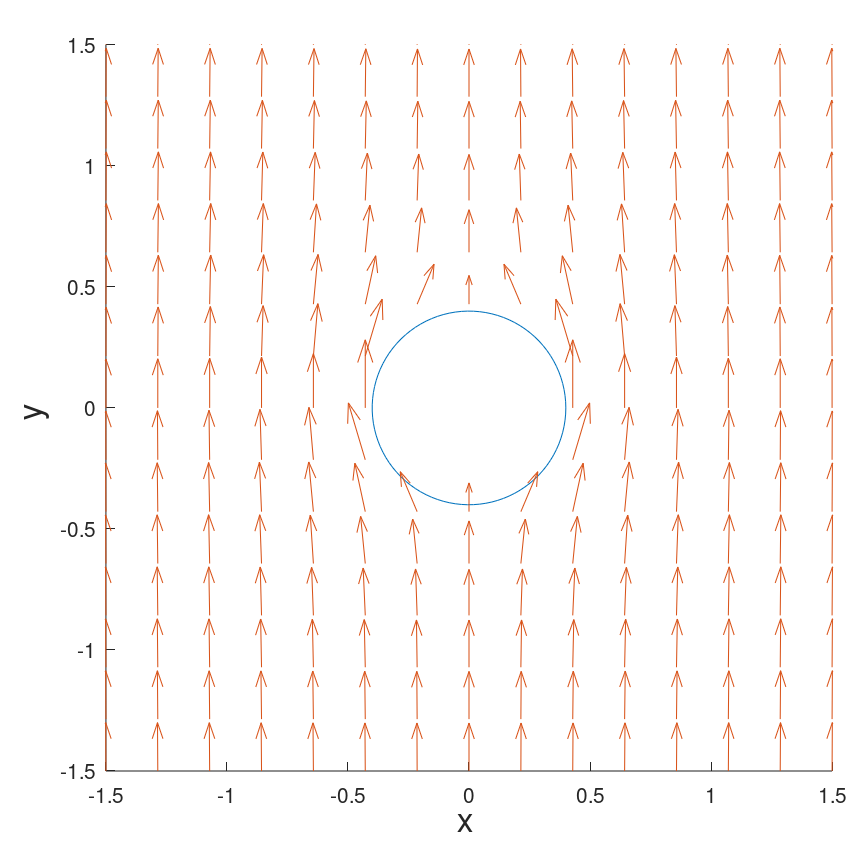
\includegraphics[height=2.5in]{images2/Streamlines.png}
\end{center}

\textcolor{mypink1}{  Obs: two streamlines can not cross each other. Why?}
\end{frame}

  %%%%%%%%%%%%%%%%%%%%%%%%%%%%%%%%%%%%%%%%%%%%%%%%%%%%%%%%%%%%%%%

\begin{frame}

We can distinguish two main types of fluid flow:
\vspace{3mm}

\begin{itemize}
\item \textcolor{mypink1}{Steady Flow:} at any one place in the fluid the velocity never 
changes \textcolor{mypink1}{$\rightarrow$ the streamlines are the fluid particles path.}
\pause
\item \textcolor{mypink1}{Non-Steady Flow:} At a given point, the velocity changes with time.
\end{itemize}

  \end{frame}

  
%%%%%%%%%%%%%%%%%%%%%%%%%%%%%%%%%%%%%%%%%%%%%%%%%%%%%%%%%%%%%%%

\begin{frame}
We are going to consider:

\pause
\vspace{5 mm}

\begin{itemize}
  \item The velocity of the flow $<<$speed of sound in the Fluid.
  \item $\rho=constant$ (incompressible fluid)
  \item steady flow.
\end{itemize}




  \end{frame}


%%%%%%%%%%%%%%%%%%%%%%%%%%%%%%%%%%%%%%%%%%%%%%%%%%%%%%%%%%%%%%%


\begin{frame}

Steady flow:

\begin{itemize}
  \item At any one place in the fluid the velocity never changes.
\pause
  \item  Fluid element moves in lines which are always tangent to the
   fluid velocity (streamlines).
\end{itemize}


  \end{frame}

%%%%%%%%%%%%%%%%%%%%%%%%%%%%%%%%%%%%%%%%%%%%%%%%%%%%%%%%%%%%%%%
\subsection{Equation of continuity}


\begin{frame}




 \begin{columns}[c]
   \column{2in}  % slides are 3in high by 5in wide
  
 \begin{center}
  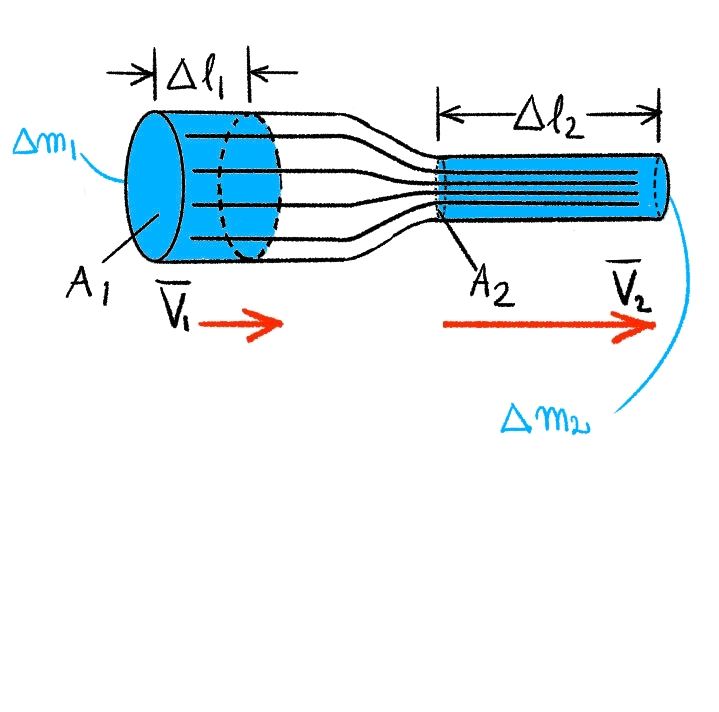
\includegraphics[height=2.5in]{images2/Fluids2.jpg}
\end{center}


   \column{2in}

\pause
\begin{itemize}
  \item Mass Flow Rate $\rightarrow \frac{\Delta m}{\Delta t}$ 
  \pause
  \item no fluid flows in or out the sides $\rightarrow \Delta m_1=\Delta m_2 $ 
  \pause

\end{itemize}

\begin{equation}
  \rightarrow \frac{\Delta m_1}{\Delta t}=\frac{\Delta m_2}{\Delta t}
\end{equation}

   \end{columns}

  \end{frame}

%%%%%%%%%%%%%%%%%%%%%%%%%%%%%%%%%%%%%%%%%%%%%%%%%%%%%%%%%%%%%%%



\begin{frame}




 \begin{columns}[c]
   \column{2in}  % slides are 3in high by 5in wide
  
 \begin{center}
  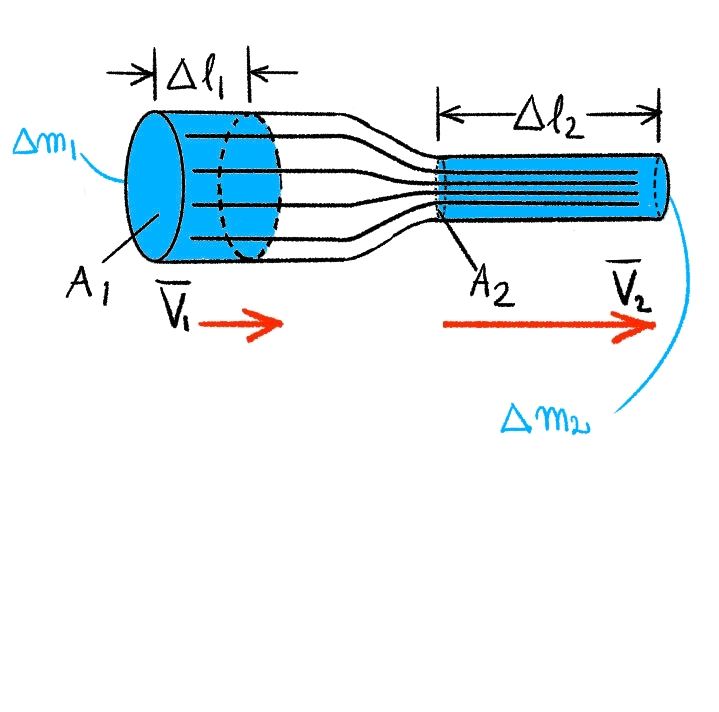
\includegraphics[height=2.5in]{images2/Fluids2.jpg}
\end{center}


   \column{2in}

\pause
\vspace{3mm}

$Vol_1= A_1 \Delta \ell_1$,
\vspace{3mm}

\pause

\begin{equation*}
   \rightarrow \frac{\Delta m_1}{\Delta t}=\frac{\rho_1 Vol_1}{\Delta t}=\frac{\rho_1A_1\Delta \ell_1}{\Delta t}
\end{equation*}
\vspace{3mm}

\pause

 $v_1=\Delta \ell_1/\Delta t$.
\vspace{3mm}

\pause
\begin{equation*}
  \rightarrow \frac{\Delta m_1}{\Delta t }=\rho_1 A_1 v_1
\end{equation*}

\vspace{3mm}

\pause



\begin{equation*}
  \rightarrow \frac{\Delta m_2}{\Delta t }=\rho_2 A_2 v_2
\end{equation*}


   \end{columns}

  \end{frame}
%%%%%%%%%%%%%%%%%%%%%%%%%%%%%%%%%%%%%%%%%%%%%%%%%%%%%%%%%%%%%%%

\begin{frame}

Then,

\begin{equation}
\rho_1A_1v_1=\rho_2A_2v_2
\end{equation}

\vspace{3mm}
\pause
This is called the \textbf{equation of continuity}.
\vspace{3mm}
If the fluid is incompressible, $\rho_2=\rho_1$, 
\pause
\begin{equation}
A_1v_1=A_2v_2
\end{equation}
\pause
$Av$ is the \textit{volume rate of flow}
\pause
\vspace{3mm}

\begin{equation*}
  \boxed{Av=constant}
\end{equation*}

  \end{frame}
%%%%%%%%%%%%%%%%%%%%%%%%%%%%%%%%%%%%%%%%%%%%%%%%%%%%%%%%%%%%%%%

\newcounter{examplef}
\setcounter{examplef}{1}

\begin{frame}
  \frametitle{Example \theexamplef }


   \begin{columns}[c]
   \column{2.3in}  % slides are 3in high by 5in wide


\textbf{Blood flow}. In humans, blood flows from the heart into the aorta, from which it passes into the major arteries. These branch into the small arteries (arterioles),
 which in turn branch into myriads of tiny capillaries. The blood returns to the heart via the veins. The radius of the aorta is about $1.2 cm$, and the blood passing through it has 
a speed of about $40 cm/s$. A typical capillary has a radius of about $4 \times 10^{-4} cm$, and blood flows through it at a speed of about $5 \times 10^ {-4} m/s$. 



   \column{2.in}

    \begin{center}
  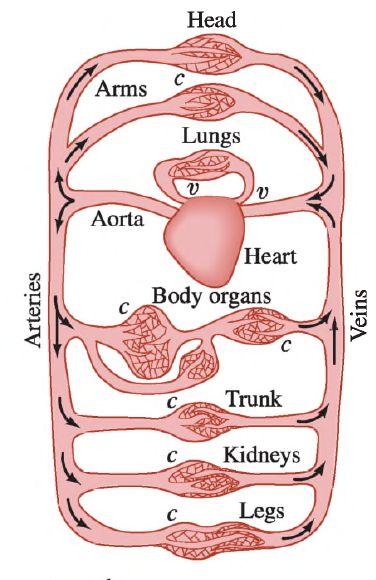
\includegraphics[height=1.9in]{images2/hb.jpg}
\end{center}
Estimate the number of capillaries that are in the body.

   \end{columns}



  \end{frame}




%%%%%%%%%%%%%%%%%%%%%%%%%%%%%%%%%%%%%%%%%%%%%%%%%%%%%%%%%%%%%%%
\subsection{Bernoulli's Equation}

\begin{frame}
\frametitle{Bernoulli's Principle}

\textit{Where the velocity of a fluid is high, the pressure is low, 
and where the velocity is low, the pressure is high.}
\pause

\vspace{5mm}

\textcolor{mypink1}{The theorem of Bernoulli is in fact nothing more than a statement of the
conservation of energy.}

  \end{frame}

%%%%%%%%%%%%%%%%%%%%%%%%%%%%%%%%%%%%%%%%%%%%%%%%%%%%%%%%%%%%%%%


% \begin{frame}

% To proof this we are going to assume,
% \vspace{3mm}

% \begin{itemize}
% \item The flow is steady and laminar
% \item The fluid is incompressible
% \item The viscosity is small enough to be ignored
% \item The fluid is flowing in a tube of variable cross section
% \end{itemize}

%   \end{frame}
%%%%%%%%%%%%%%%%%%%%%%%%%%%%%%%%%%%%%%%%%%%%%%%%%%%%%%%%%%%%%%%


\begin{frame}


   \begin{columns}[c]
   \column{1.8in}  % slides are 3in high by 5in wide
  

  \begin{center}
  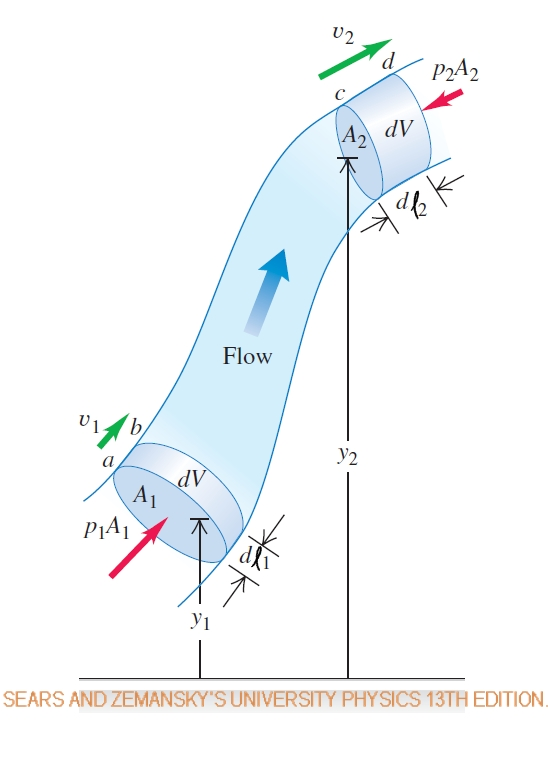
\includegraphics[height=3.in]{images2/Bernoulli_SZ.jpg}
\end{center}



   \column{2.2in}


The work done at $A_1$ is,
\begin{equation}
W_1=F_1\Delta \ell_1=P_1 A_1 \Delta \ell_1
\end{equation}
\pause
At area $A_2$, 
\pause
\begin{equation}
W_2=-P_2 A_2 \Delta \ell_2
\end{equation}
\pause
The work done by gravity is,
\pause
\begin{equation}
W_3=-mg(y_2-y_1)
\end{equation}





   \end{columns}

\pause
\begin{eqnarray*}
W&=&W_1+W_2+W_3\\
&=&P_1A_1\Delta \ell_1-P_2 A_2 \Delta \ell_2-mg(y_2-y_1)\\
\end{eqnarray*}



  \end{frame}


%%%%%%%%%%%%%%%%%%%%%%%%%%%%%%%%%%%%%%%%%%%%%%%%%%%%%%%%%%%%%%%


\begin{frame}


\begin{equation*}
W=\Delta E_k=\frac{1}{2}mv^2_2-\frac{1}{2}mv^2_1
\end{equation*}
\pause
then,


\begin{equation*}
\frac{1}{2}mv^2_2-\frac{1}{2}mv^2_1=P_1A_1\Delta \ell_1-P_2 A_2 \Delta \ell_2-mg(y_2-y_1)
\end{equation*}
\pause
$m_1=m_2=m$ Incompressible fluid $\rho_1=\rho_2\rightarrow V_1=V_2$
\pause
\begin{equation*}
\rightarrow A_1\Delta \ell_1=A_2 \Delta \ell_2
\end{equation*}
\pause
\begin{equation*}
\rightarrow m=\rho A_1\Delta \ell_1=\rho A_2\Delta \ell_2
\end{equation*}
\pause
Then,

\begin{equation*}
\frac{1}{2}\rho v^2_2-\frac{1}{2}\rho v^2_1=P_1-P_2-\rho g(y_2-y_1)
\end{equation*}



  \end{frame}


%%%%%%%%%%%%%%%%%%%%%%%%%%%%%%%%%%%%%%%%%%%%%%%%%%%%%%%%%%%%%%%


\begin{frame}


Reordering the expression,
\vspace{3mm}
\pause
\begin{equation*}
\frac{1}{2}\rho v^2_2+P_2+ \rho gy_2=\frac{1}{2} \rho v^2_1+P_1+ \rho gy_1 
\end{equation*}
\pause
\vspace{3mm}
\pause
This is \textbf{Bernoulli’s equation}. Since points 1 and 2 can be any two points along a
tube of flow, Bernoulli’s equation can be written as
\vspace{3mm}
\pause
\begin{equation}
\boxed{\frac{1}{2}\rho v^2+P+ \rho gy=constant}
\end{equation}



  \end{frame}
%%%%%%%%%%%%%%%%%%%%%%%%%%%%%%%%%%%%%%%%%%%%%%%%%%%%%%%%%%%%%%%


\begin{frame}


if the velocities are zero, 
\pause
\begin{equation*}
P_2+ \rho gy_2=P_1+ \rho gy_1 
\end{equation*}

\pause
\begin{equation}
P_2-P_1=-\rho g(y_2-y_1) \leftarrow Hydrostatic~equation
\end{equation}
\vspace{3mm}



  \end{frame}

%%%%%%%%%%%%%%%%%%%%%%%%%%%%%%%%%%%%%%%%%%%%%%%%%%%%%%%%%%%%%%%


\stepcounter{examplef}

\begin{frame}
  \frametitle{Example \theexamplef }



Calculate the velocity, $v_1$, of a liquid flowing out of a spigot at the bottom of a reservoir.
\vspace{3mm}

  \begin{center}
  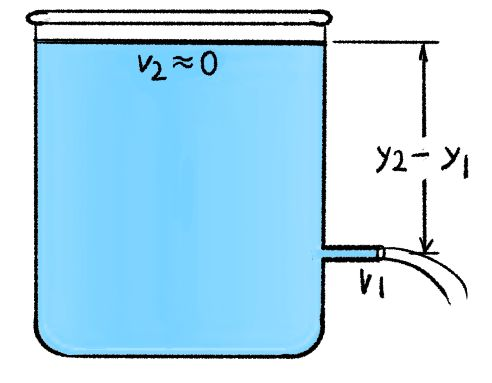
\includegraphics[height=1.7in]{images2/Bernoulli2.jpg}
\end{center}
\pause 
\textcolor{mypink1}{The liquid leaves the spigot with the same speed that a
freely falling object would attain if falling from the same height.}
  \end{frame}

 
  %%%%%%%%%%%%%%%%%%%%%%%%%%%%%%%%%%%%%%%%%%%%%%%%%%%%%%%%%%%%%%%

  \stepcounter{examplef}

  \begin{frame}
    \frametitle{Example \theexamplef }
    Figure \ref{venturi} shows a Venturi meter, used to measure flow speed in
    a pipe. Derive an expression for the flow speed in terms of the
    cross-sectional areas and and the difference in height $h$ of
    the liquid levels in the two vertical tubes.

    \begin{figure}[h!]
      \begin{center}
        \includegraphics[height=2.in]{images2/venturi.jpg}
        \label{venturi}
      \end{center}
    \end{figure}

    

    \end{frame}

      %%%%%%%%%%%%%%%%%%%%%%%%%%%%%%%%%%%%%%%%%%%%%%%%%%%%%%%%%%%%%%%

  \stepcounter{examplef}

  \begin{frame}
\textcolor{mypink1}{Solved in whiteboar}


    \begin{columns}[c]
      \column{2in}  % slides are 3in high by 5in wide
   
      \begin{figure}[h!]
        \begin{center}
          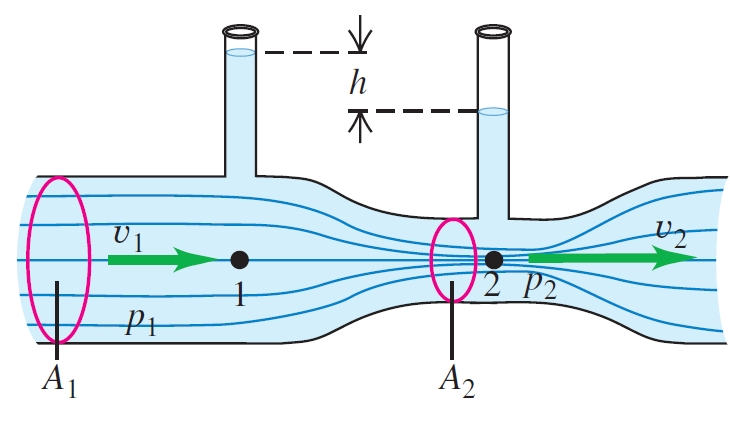
\includegraphics[height=1.3in]{images2/venturi2.jpg}
        \end{center}
      \end{figure}
  
      \column{2in}
   
   
      \end{columns}
   

    \end{frame}

    %%%%%%%%%%%%%%%%%%%%%%%%%%%%%%%%%%%%%%%%%%%%%%%%%%%%%%%%%%%%%%%
  
\stepcounter{examplef}

\begin{frame}
  \frametitle{Example \theexamplef }
  In 1993 the radius of Hurricane Emily was about
  350 km.
The wind speed near the center (“eye”) of a hurricane,
  whose radius is  $30~km$, reaches about $200~km/h$. As air
  swirled in from the rim of the hurricane toward the eye, its angular
  momentum remained roughly constant. (a) Estimate the wind
speed at the rim of the hurricane. (b) Estimate the pressure difference
at the earth’s surface between the eye and the rim.  
Where is the pressure greater? 

  \end{frame}
      %%%%%%%%%%%%%%%%%%%%%%%%%%%%%%%%%%%%%%%%%%%%%%%%%%%%%%%%%%%%%%%
  
\stepcounter{examplef}

\begin{frame}
  \frametitle{Example \theexamplef }
  \textcolor{mypink1}{Solved in whiteboar}

  \end{frame}

    %%%%%%%%%%%%%%%%%%%%%%%%%%%%%%%%%%%%%%%%%%%%%%%%%%%%%%%%%%%%%%%


  \stepcounter{examplef}

      
  

  \begin{frame}
    \frametitle{Example \theexamplef }
  
 
    A siphon is a convenient
    device for removing liquids from containers. To establish the flow,
    the tube must be initially filled with fluid. Let the fluid have density $\rho$
    and let the atmospheric pressure be $P_{atm}$. Assume that the
    cross-sectional area of the tube is the same at all points along it. 


    \begin{center}
      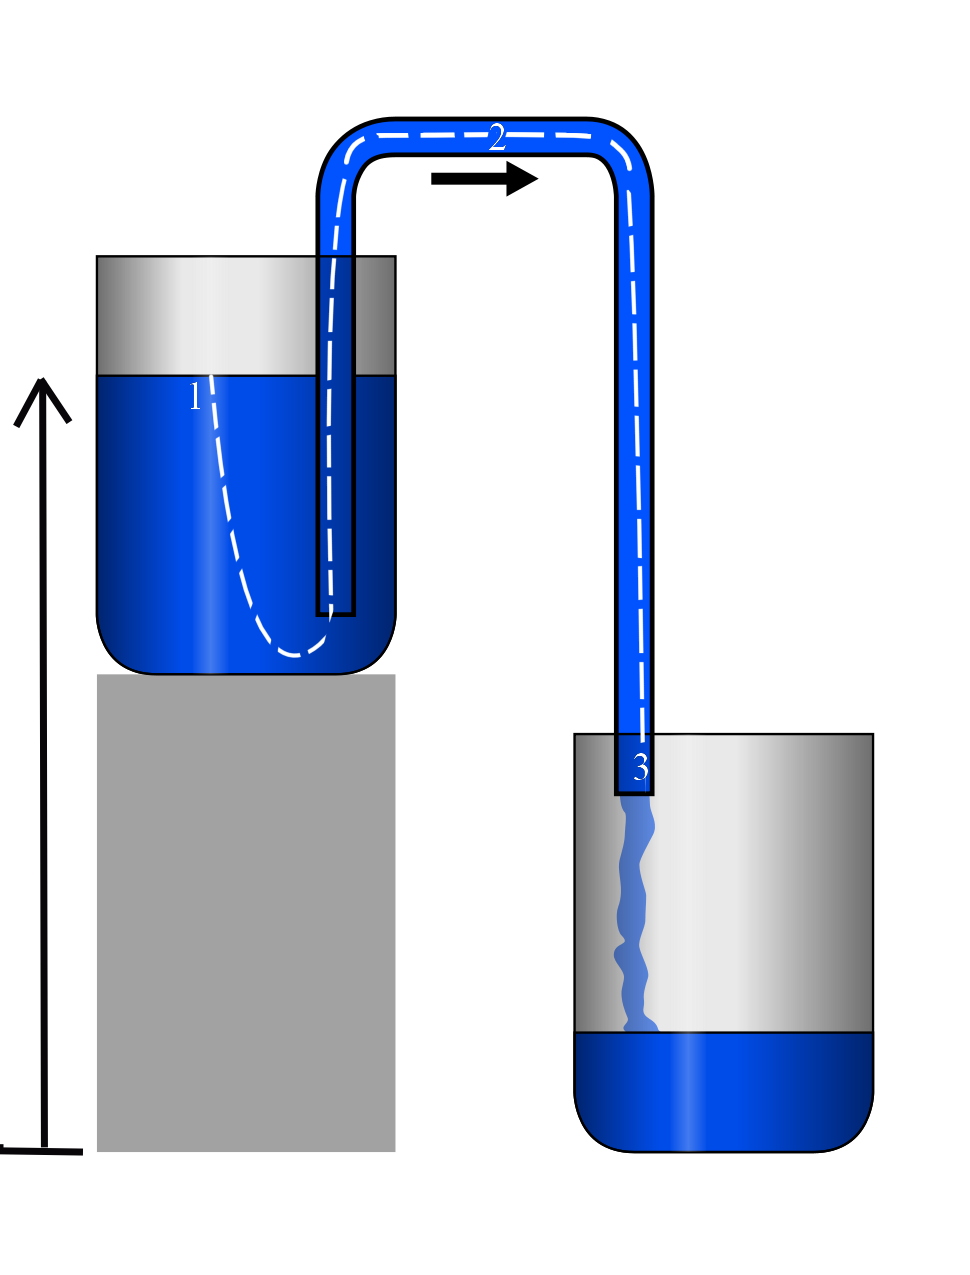
\includegraphics[height=1.7in]{images2/Syphon.png}
    \end{center}


  
    \end{frame}



    %%%%%%%%%%%%%%%%%%%%%%%%%%%%%%%%%%%%%%%%%%%%%%%%%%%%%%%%%%%%%%%


    \begin{frame}
  \frametitle{Example \theexamplef }



  \begin{enumerate}
    \item If the lower end of the siphon is at a distance h below the surface
    of the liquid in the container, what is the speed of the fluid as it
    flows out the lower end of the siphon? (Assume that the container
    has a very large diameter, and ignore any effects of viscosity.
    \item A curious feature of a siphon is that the fluid initially flows
    “uphill.” What is the greatest height H that the high point of the
    tube can have if flow is still to occur?
  \end{enumerate}
  

  \end{frame}

    %%%%%%%%%%%%%%%%%%%%%%%%%%%%%%%%%%%%%%%%%%%%%%%%%%%%%%%%%%%%%%%



    \begin{frame}


      \begin{columns}[c]
        \column{2in}  % slides are 3in high by 5in wide
     
        \begin{center}
          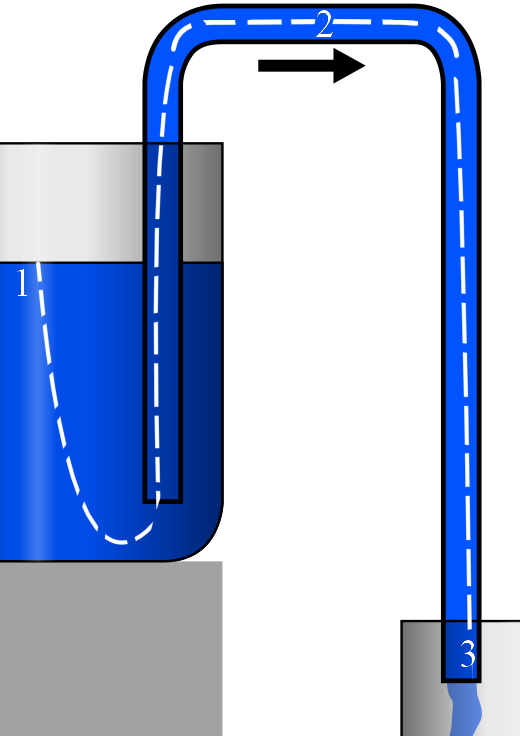
\includegraphics[height=2.in]{images2/Syphon_streamline.png}
        \end{center}

        \column{2.8in}
     
        \textcolor{mypink1}{  (1) 
        \begin{eqnarray*}
        P_0+\rho g h&=&P_0+\frac{1}{2} \rho v_3^2\\
          \pause
          \rightarrow v_3&=& \boxed{\sqrt{2gh}}\\
        \end{eqnarray*}
              }

        \end{columns}
     


    
      \end{frame}


%%%%%%%%%%%%%%%%%%%%%%%%%%%%%%%%%%%%%%%%%%%%%%%%%%%%%%%%%%%%%%%


\begin{frame}


  \begin{columns}[c]
    \column{1.5in}  % slides are 3in high by 5in wide
 
    \begin{center}
      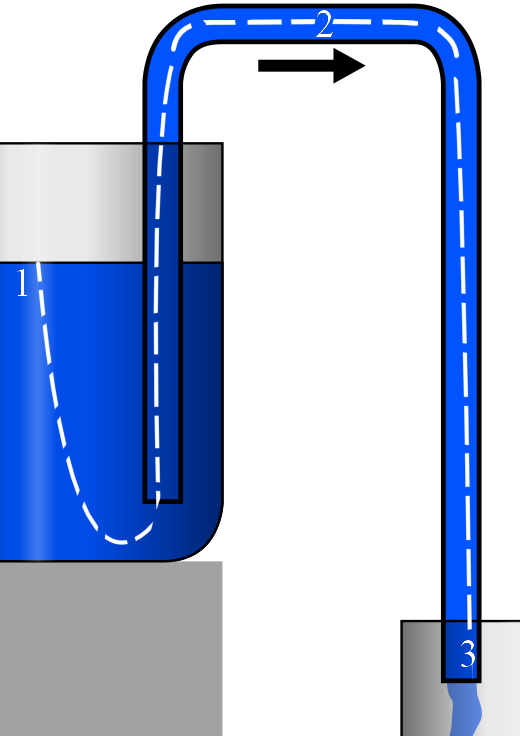
\includegraphics[height=1.5in]{images2/Syphon_streamline.png}
    \end{center}

    \column{3.9in}
 
    \textcolor{mypink1}{  (2) 
    \begin{eqnarray*}
     Bernoulli~ (2)&=&Bernoulli~  (3) \\
     \pause
       P_2+\frac{1}{2}\rho v_2^2+\rho g (H+h)&=&P_0+\frac{1}{2}\rho v_3^2 \\
       \pause
       v_2A_2&=&v_3A_3\\
       \pause
       \rightarrow v_2&=&v_3\\
       \pause
       \rightarrow P_2+\frac{1}{2}\rho v_3^2+\rho g (H+h)&=&P_0+\frac{1}{2}\rho v_3^2\\
       \pause
      \rightarrow H&=& \frac{P_0-P_2}{\rho g}-h\\
    \end{eqnarray*}
    \pause
    \begin{equation*}
      min~~P_2=0~\rightarrow H_{max}=\boxed{\frac{P_0}{\rho g}-h}
    \end{equation*}
          }

    \end{columns}
 



  \end{frame}


%%%%%%%%%%%%%%%%%%%%%%%%%%%%%%%%%%%%%%%%%%%%%%%%%%%%%%%%%%%%%%%



\begin{frame}



\textbf{Conceptual example: How does a Perfume Atomizer work?}

\vspace{5mm}



   \begin{columns}[c]
   \column{2in}  % slides are 3in high by 5in wide
  
  \begin{center}
  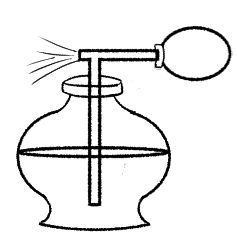
\includegraphics[height=1.7in]{images2/aspersor.jpg}
\end{center}



   \column{2in}

\pause

The pressure in the air blown at high speed across the top of
the vertical tube of a perfume atomizer is less than the normal air
pressure acting on the surface of the liquid in the bowl. Thus atmospheric pressure
in the bowl pushes the perfume up the tube because of the lower pressure at the
top.


   \end{columns}



 \end{frame}





%%%%%%%%%%%%%%%%%%%%%%%%%%%%%%%%%%%%%%%%%%%%%%%%%%%%%%%%%%%%%%%


\subsection{viscosity}

\begin{frame}

\frametitle{Viscosity}
Real Fluids have certain amount of internal friction called $\textbf{viscosity}$. 
It is a frictional force between adjacent layers of fluid.
\vspace{3mm}

\pause
The origin of the viscosity is,

\begin{itemize}
\item In fluids, electrical cohesive forces between the molecules. \pause\textcolor{mypink1}{it decrases with T}
\pause
\item In gases, collisions between the molecules. \pause\textcolor{mypink1}{it increases with T}
\end{itemize}
\vspace{3mm}

\pause

The viscosity can be expressed quantitatively by a \textit{coefficient of viscosity} $\eta$


 \end{frame}

%%%%%%%%%%%%%%%%%%%%%%%%%%%%%%%%%%%%%%%%%%%%%%%%%%%%%%%%%%%%%%%


\begin{frame}

\frametitle{Viscosity}

\textcolor{mypink1}{How do we calculate it?}
\pause

  \begin{center}
  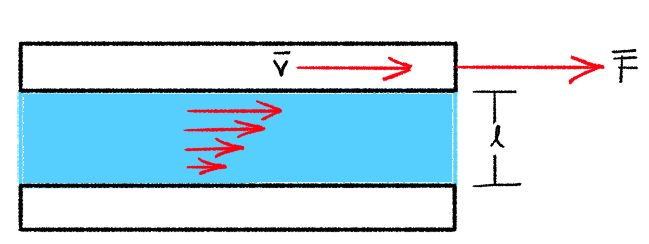
\includegraphics[height=1.in]{images2/vicosity.jpg}
\end{center}

\pause
\begin{equation}
F=\propto A \frac{v}{\ell} 
\end{equation}

\pause
\begin{equation}
F=\eta A \frac{v}{\ell} \rightarrow \eta=\boxed{\frac{F\ell}{Av} }
\end{equation}
\pause

The unit of $\eta$ is $N\cdot s/m^2=Pa\cdot s$

 \end{frame}



%%%%%%%%%%%%%%%%%%%%%%%%%%%%%%%%%%%%%%%%%%%%%%%%%%%%%%%%%%%%%%%



\begin{frame}

  \frametitle{Viscosity}
  
  \textcolor{mypink1}{How do we calculate it?}

  
    \begin{center}
    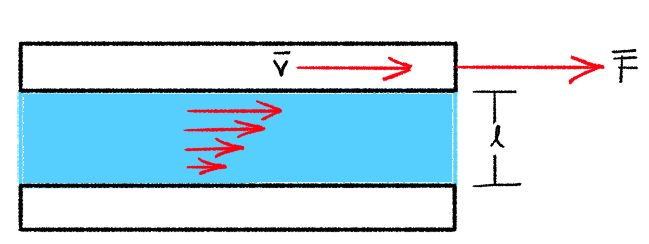
\includegraphics[height=1.in]{images2/vicosity.jpg}
  \end{center}


  There
  is always a thin boundary layer of fluid near the surface, in which the fluid is
  nearly at rest with respect to the surface. That’s why dust particles can cling to a fan blade even when it is rotating rapidly
   \end{frame}


%%%%%%%%%%%%%%%%%%%%%%%%%%%%%%%%%%%%%%%%%%%%%%%%%%%%%%%%%%%%%%%


\begin{frame}




 \begin{center}
  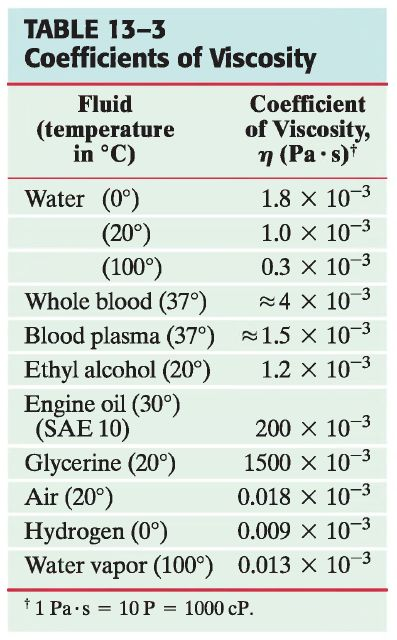
\includegraphics[height=2.6in]{images2/viscosity.jpg}
\end{center}


 \end{frame}


%%%%%%%%%%%%%%%%%%%%%%%%%%%%%%%%%%%%%%%%%%%%%%%%%%%%%%%%%%%%%%%


\begin{frame}

  \textcolor{mypink1}{Viscous fluid in a cylindrical pipe}:
  \pause \textit{"The motion is like a lot of concentric tubes sliding relative to one another".}
  
  
   \begin{center}
    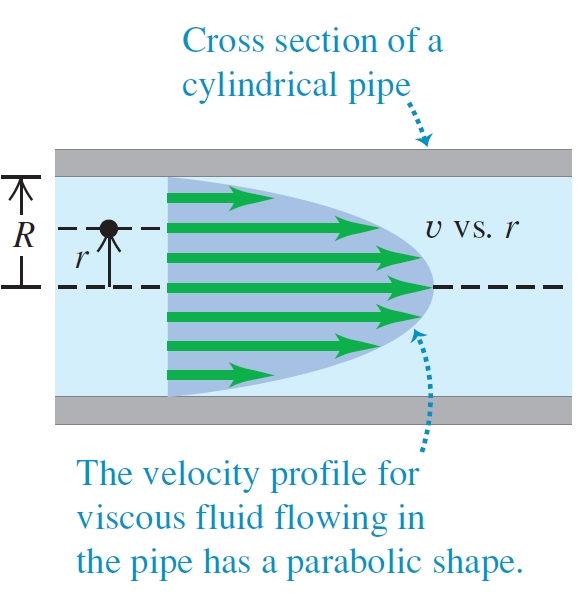
\includegraphics[height=2.2in]{images2/viscosity2.jpg}
  \end{center}
  
  \pause
  A pressure difference $\propto L/R^4$ is required to sustain the motion.
  
   \end{frame}
  %%%%%%%%%%%%%%%%%%%%%%%%%%%%%%%%%%%%%%%%%%%%%%%%%%%%%%%%%%%%%%%


   \begin{frame}
    \begin{itemize}
      \item    This simple relationship, $\propto L/R^4$,
      explains the connection between a high-cholesterol diet (which tends to narrow
      the arteries) and high blood pressure.
      \pause
      \item That’s  why you have to keep squeezing a tube of toothpaste or a packet of ketchup
       to keep the fluid coming out of its container.
    \end{itemize}


\end{frame}

%%%%%%%%%%%%%%%%%%%%%%%%%%%%%%%%%%%%%%%%%%%%%%%%%%%%%%%%%%%%%%%

%\begin{frame}

%\frametitle{Viscosity}




%\textbf{Poiseuille's Equation}
%\vspace{3mm}

%If a fluid had no viscosity, it could flow through a level tube or pipe without a force
%being applied. If there is firction, we need a froce to move the fluid.
%\vspace{3mm}


%Flow rate of an incompressible fluid undergoing laminar
%flow in a cylindrical tube:

%\vspace{3mm}

%\begin{equation}
%Q=\frac{\pi R^4(P_1-P_2)}{8\eta \ell}
%\end{equation}


 %\end{frame}


%%%%%%%%%%%%%%%%%%%%%%%%%%%%%%%%%%%%%%%%%%%%%%%%%%%%%%%%%%%%%%%

\begin{frame}



  \textbf{Coanda effect}
  
    \begin{center}
    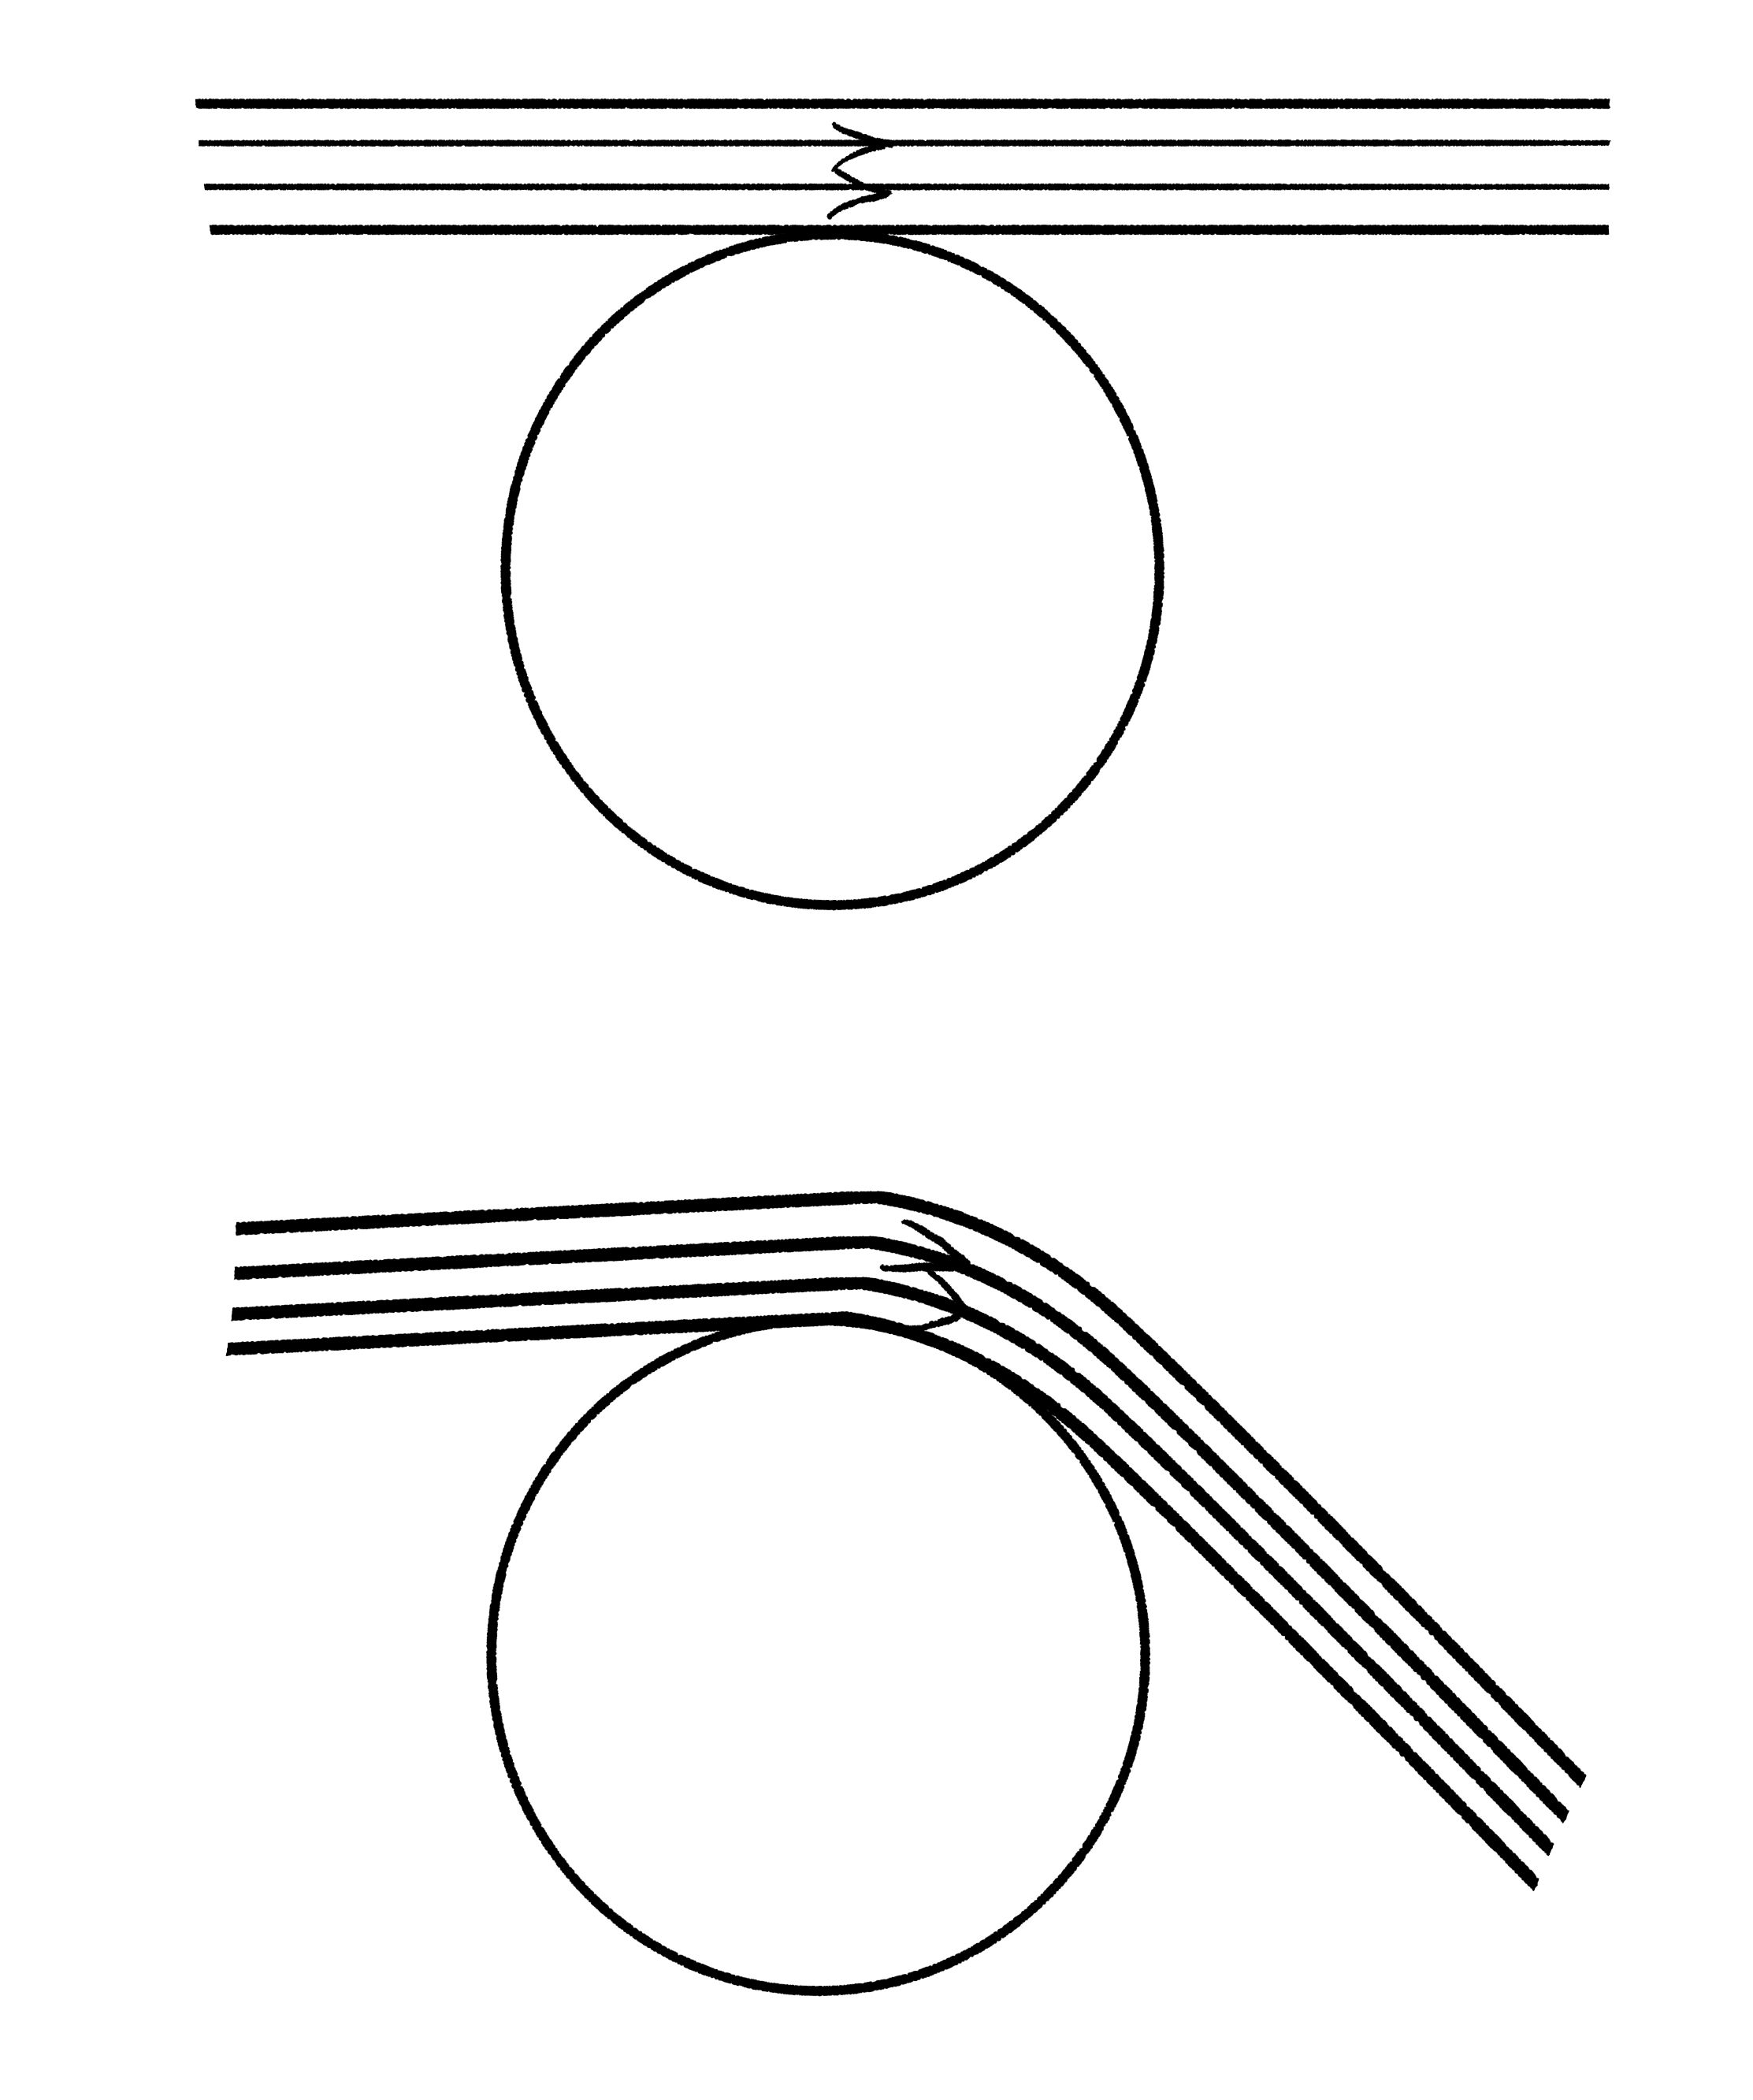
\includegraphics[height=1.7in]{images2/coanda.jpg}
  \end{center}
  
  
  \url{https://www.youtube.com/watch?v=NvzXKZNJ7ZU&t=4s}
  
   \end{frame}
  
  %%%%%%%%%%%%%%%%%%%%%%%%%%%%%%%%%%%%%%%%%%%%%%%%%%%%%%%%%%%%%%%
  
  \begin{frame}
  
  
  
    \textbf{ Airplane Wings and Dynamic Lift}
  \vspace{3mm}
  
  
    \begin{center}
    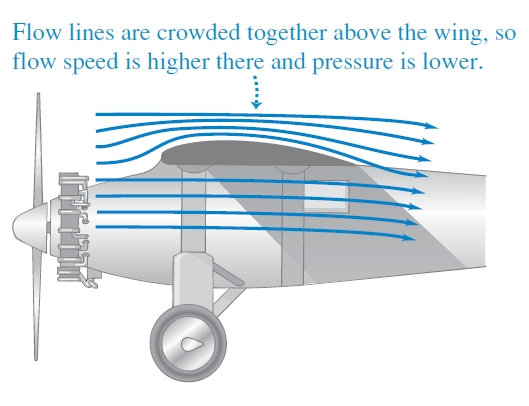
\includegraphics[height=1.8in]{images2/plane0.jpg}
  \end{center}
  
  
   \end{frame}
%%%%%%%%%%%%%%%%%%%%%%%%%%%%%%%%%%%%%%%%%%%%%%%%%%%%%%%%%%%%%%%


\begin{frame}

  \frametitle{Surface Tension and Capillarity}
  
  \pause


  
  \begin{columns}[c]
    \column{2in}  % slides are 3in high by 5in wide
 
    \begin{center}
      \includegraphics[height=1.8in]{images2/avispa.jpg}
    \end{center}
    
    \column{2in}
 
   
Why a body with a density several times the density of water cans rest \textit{atop} the water surface?
  
    \end{columns}
  
  
   \end{frame}

%%%%%%%%%%%%%%%%%%%%%%%%%%%%%%%%%%%%%%%%%%%%%%%%%%%%%%%%%%%%%%%


\begin{frame}

\frametitle{Surface Tension and Capillarity}



The particles that make up the liquid are in constant random motion.

  \begin{center}
  \includegraphics[height=1.7in]{images2/surfacet1.jpg}
\end{center}





 \end{frame}

%%%%%%%%%%%%%%%%%%%%%%%%%%%%%%%%%%%%%%%%%%%%%%%%%%%%%%%%%%%%%%%


\begin{frame}

\frametitle{Surface Tension and Capillarity}

Do the particles at the surface form a random irregular surface?

  \begin{center}
  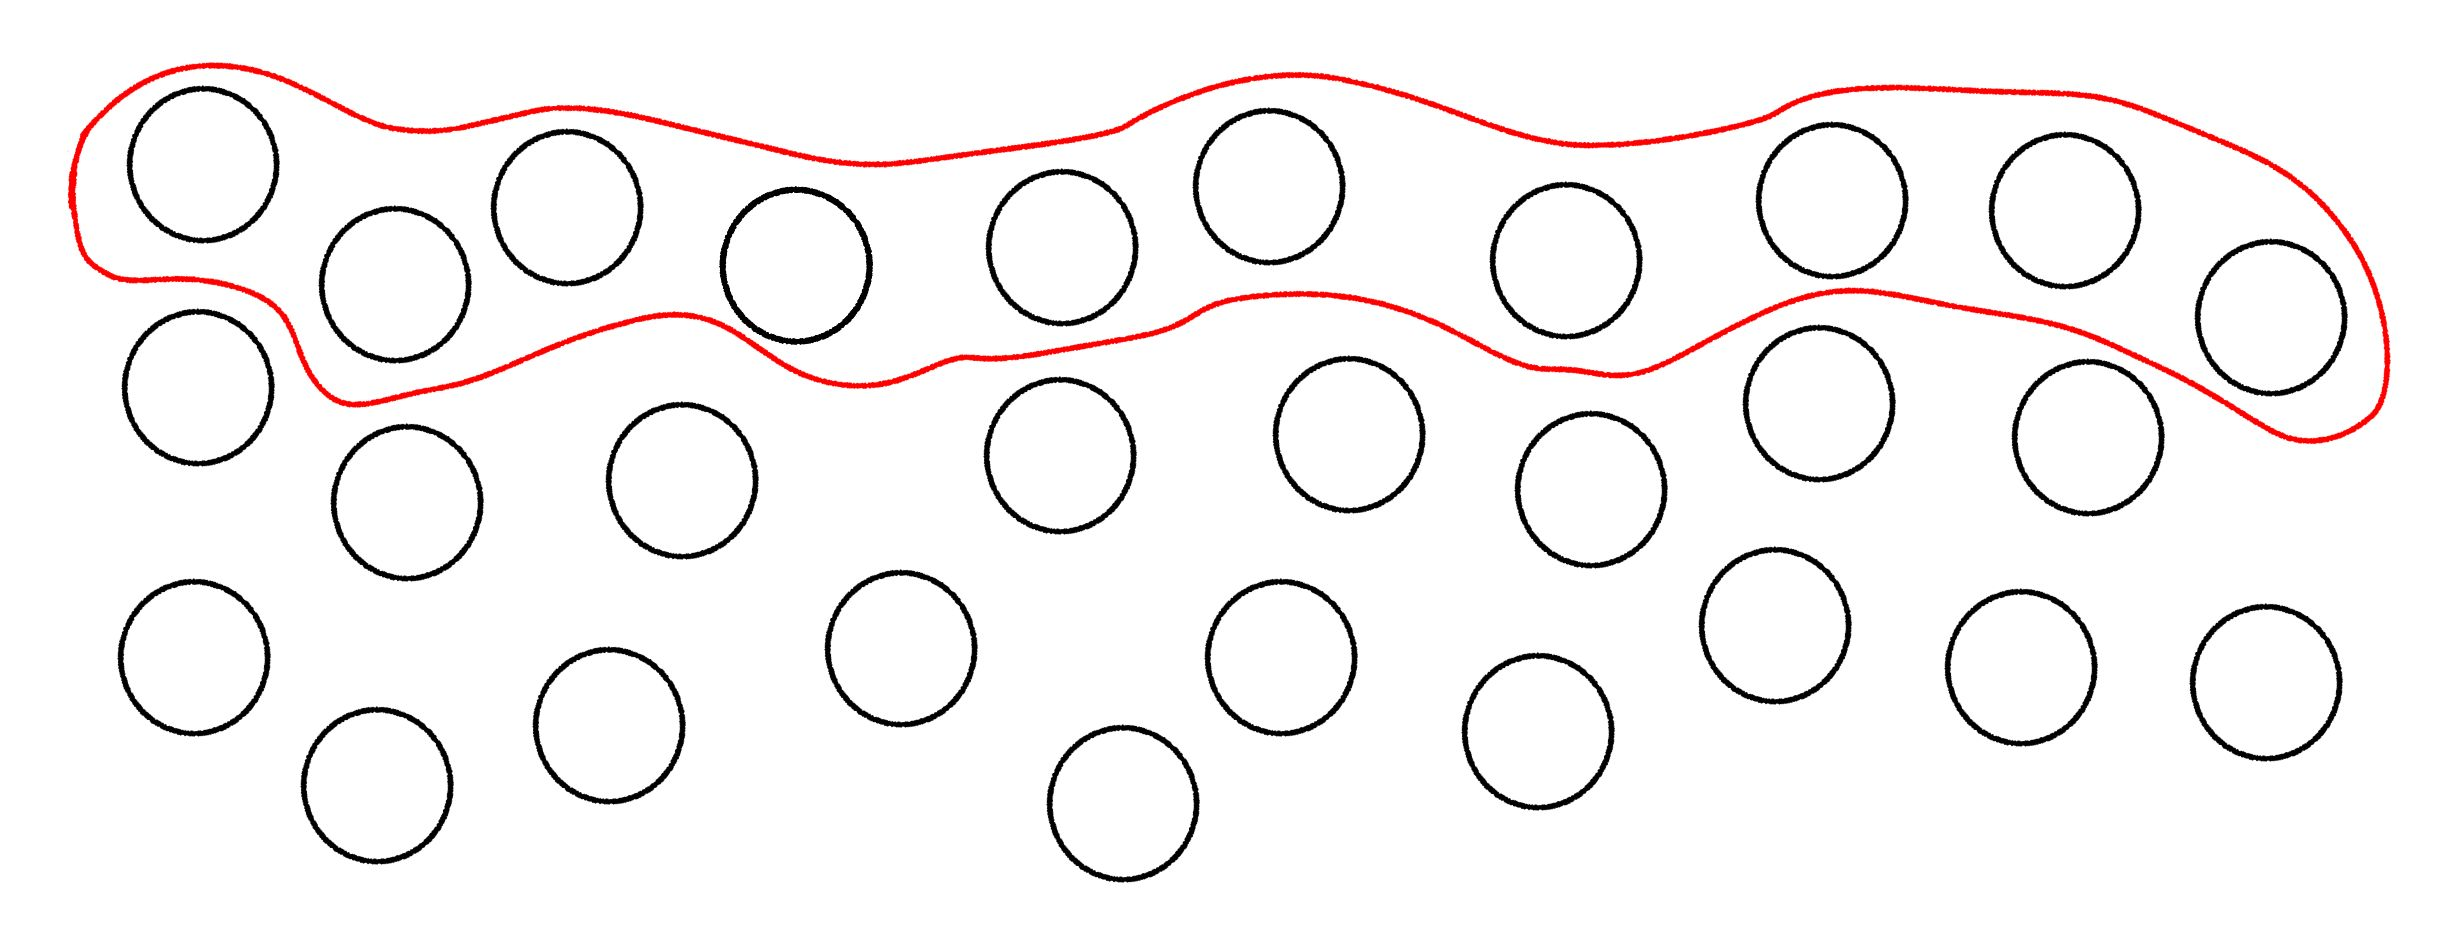
\includegraphics[height=1.7in]{images2/surfacet4.jpg}
\end{center}





 \end{frame}

%%%%%%%%%%%%%%%%%%%%%%%%%%%%%%%%%%%%%%%%%%%%%%%%%%%%%%%%%%%%%%%


\begin{frame}

\frametitle{Surface Tension and Capillarity}

Molecules in a liquid are attracted by
neighboring molecules.



  \begin{center}
  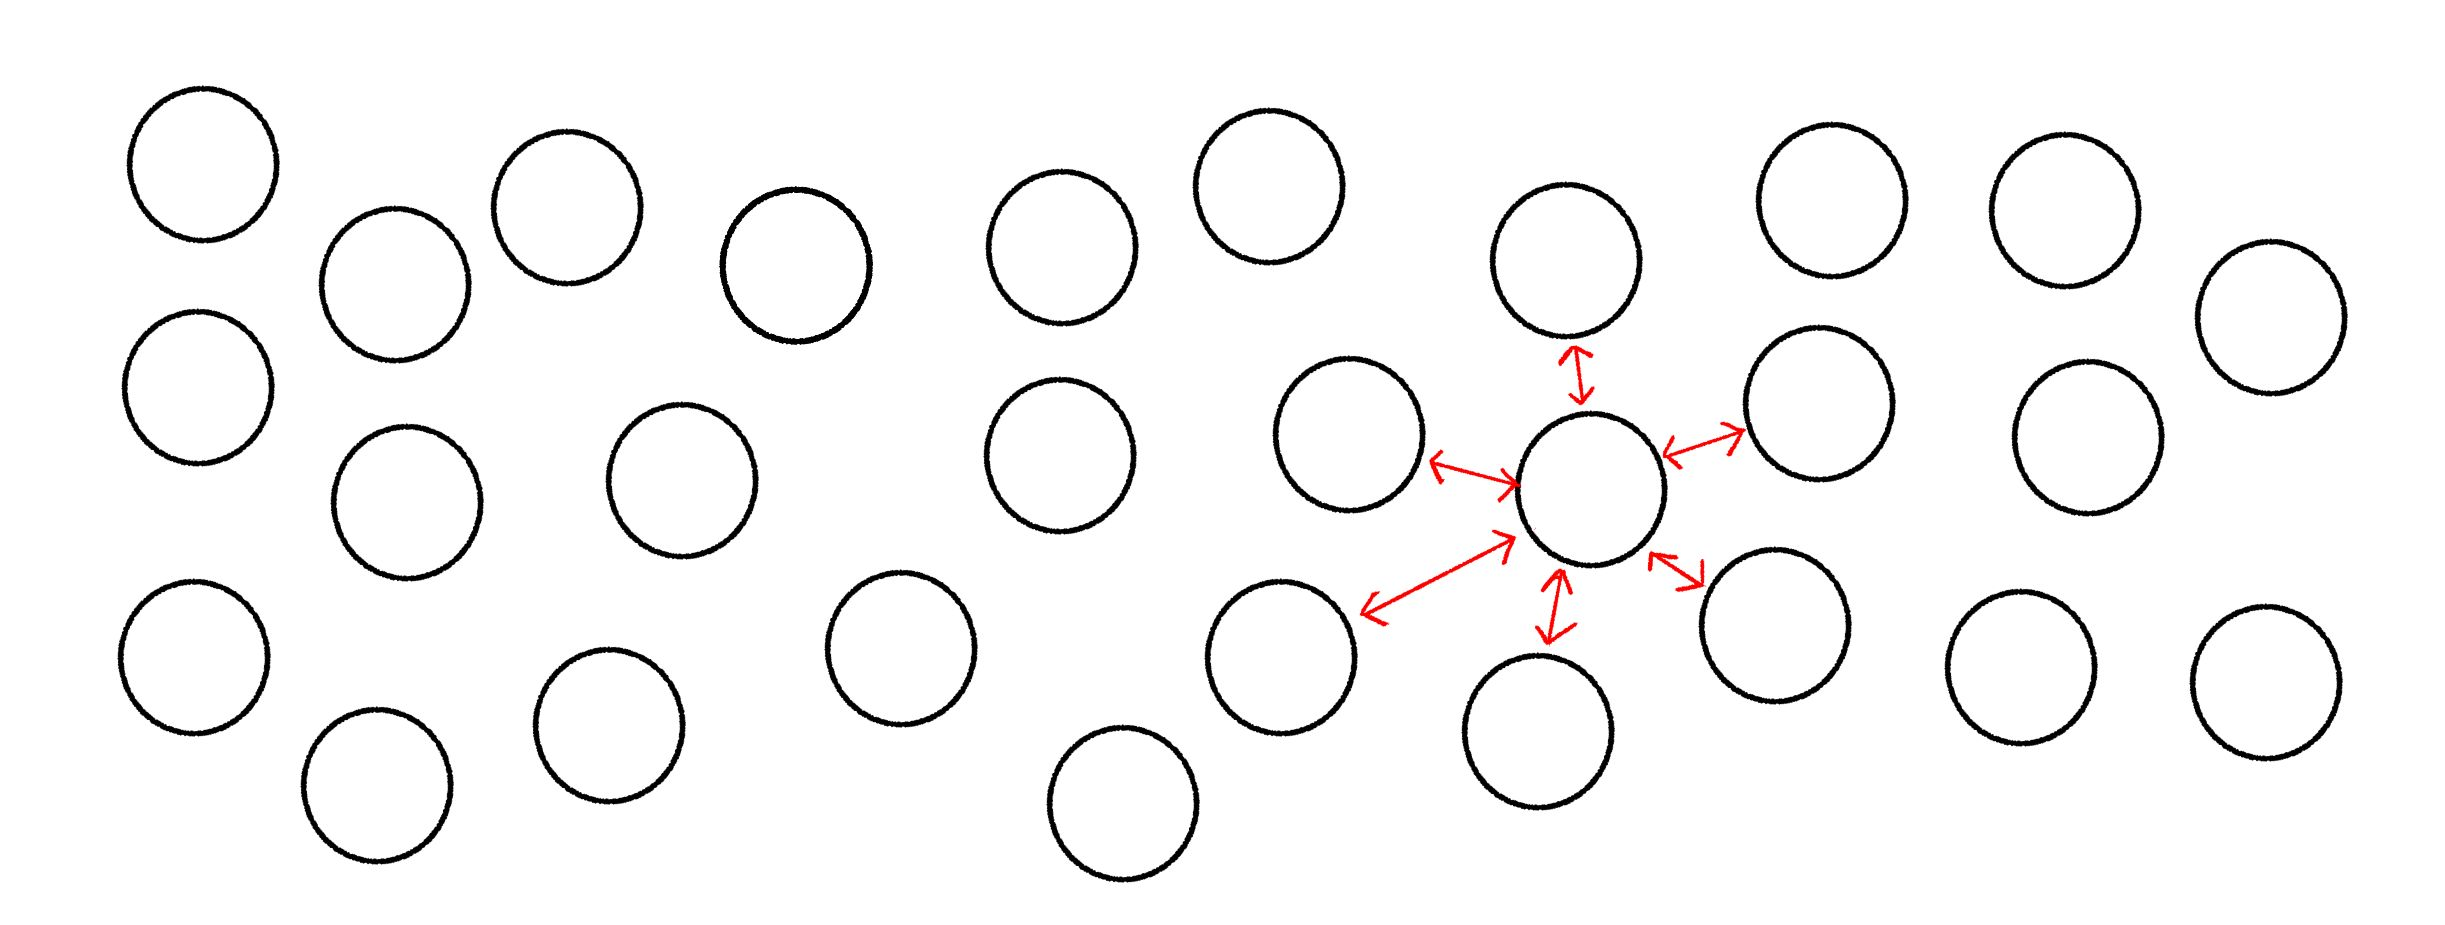
\includegraphics[height=1.7in]{images2/surfacet2.jpg}
\end{center}


\textcolor{red}{Molecules in the
interior are equally
attracted in all
directions.}


 \end{frame}

%%%%%%%%%%%%%%%%%%%%%%%%%%%%%%%%%%%%%%%%%%%%%%%%%%%%%%%%%%%%%%%


\begin{frame}

\frametitle{Surface Tension and Capillarity}

Molecules in a liquid are attracted by
neighboring molecules.

  \begin{center}
  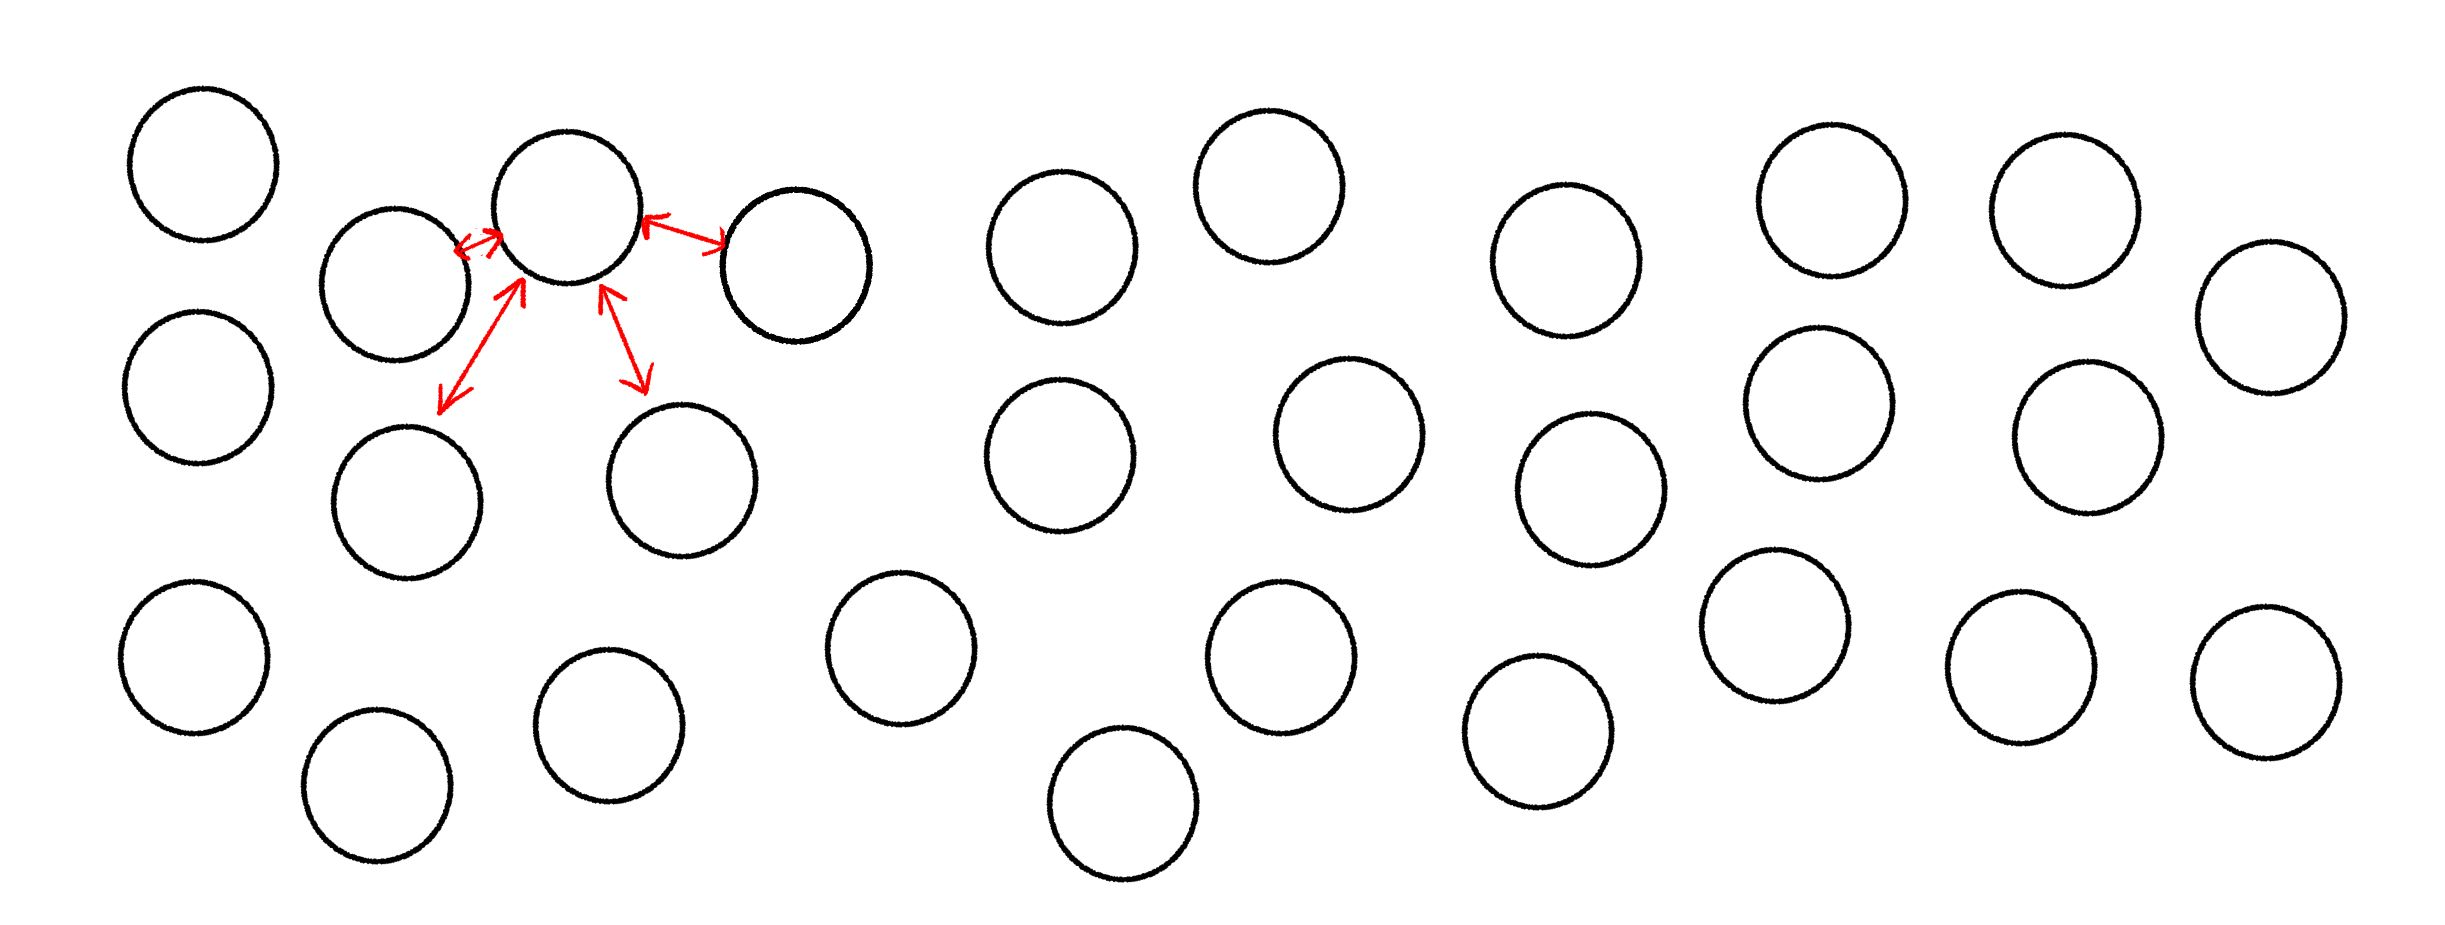
\includegraphics[height=1.7in]{images2/surfacet3.jpg}
\end{center}


\textcolor{red}{Molecules in the
interior are equally
attracted in all
directions.}



 \end{frame}

%%%%%%%%%%%%%%%%%%%%%%%%%%%%%%%%%%%%%%%%%%%%%%%%%%%%%%%%%%%%%%%


\begin{frame}

\frametitle{Surface Tension and Capillarity}

Surface molecules form a much smoother surface.
\vspace{3mm}
\pause
Surface Molecules are compressed and minimizes the surface $\rightarrow$ \pause Higher energy at the surface.

  \begin{center}
  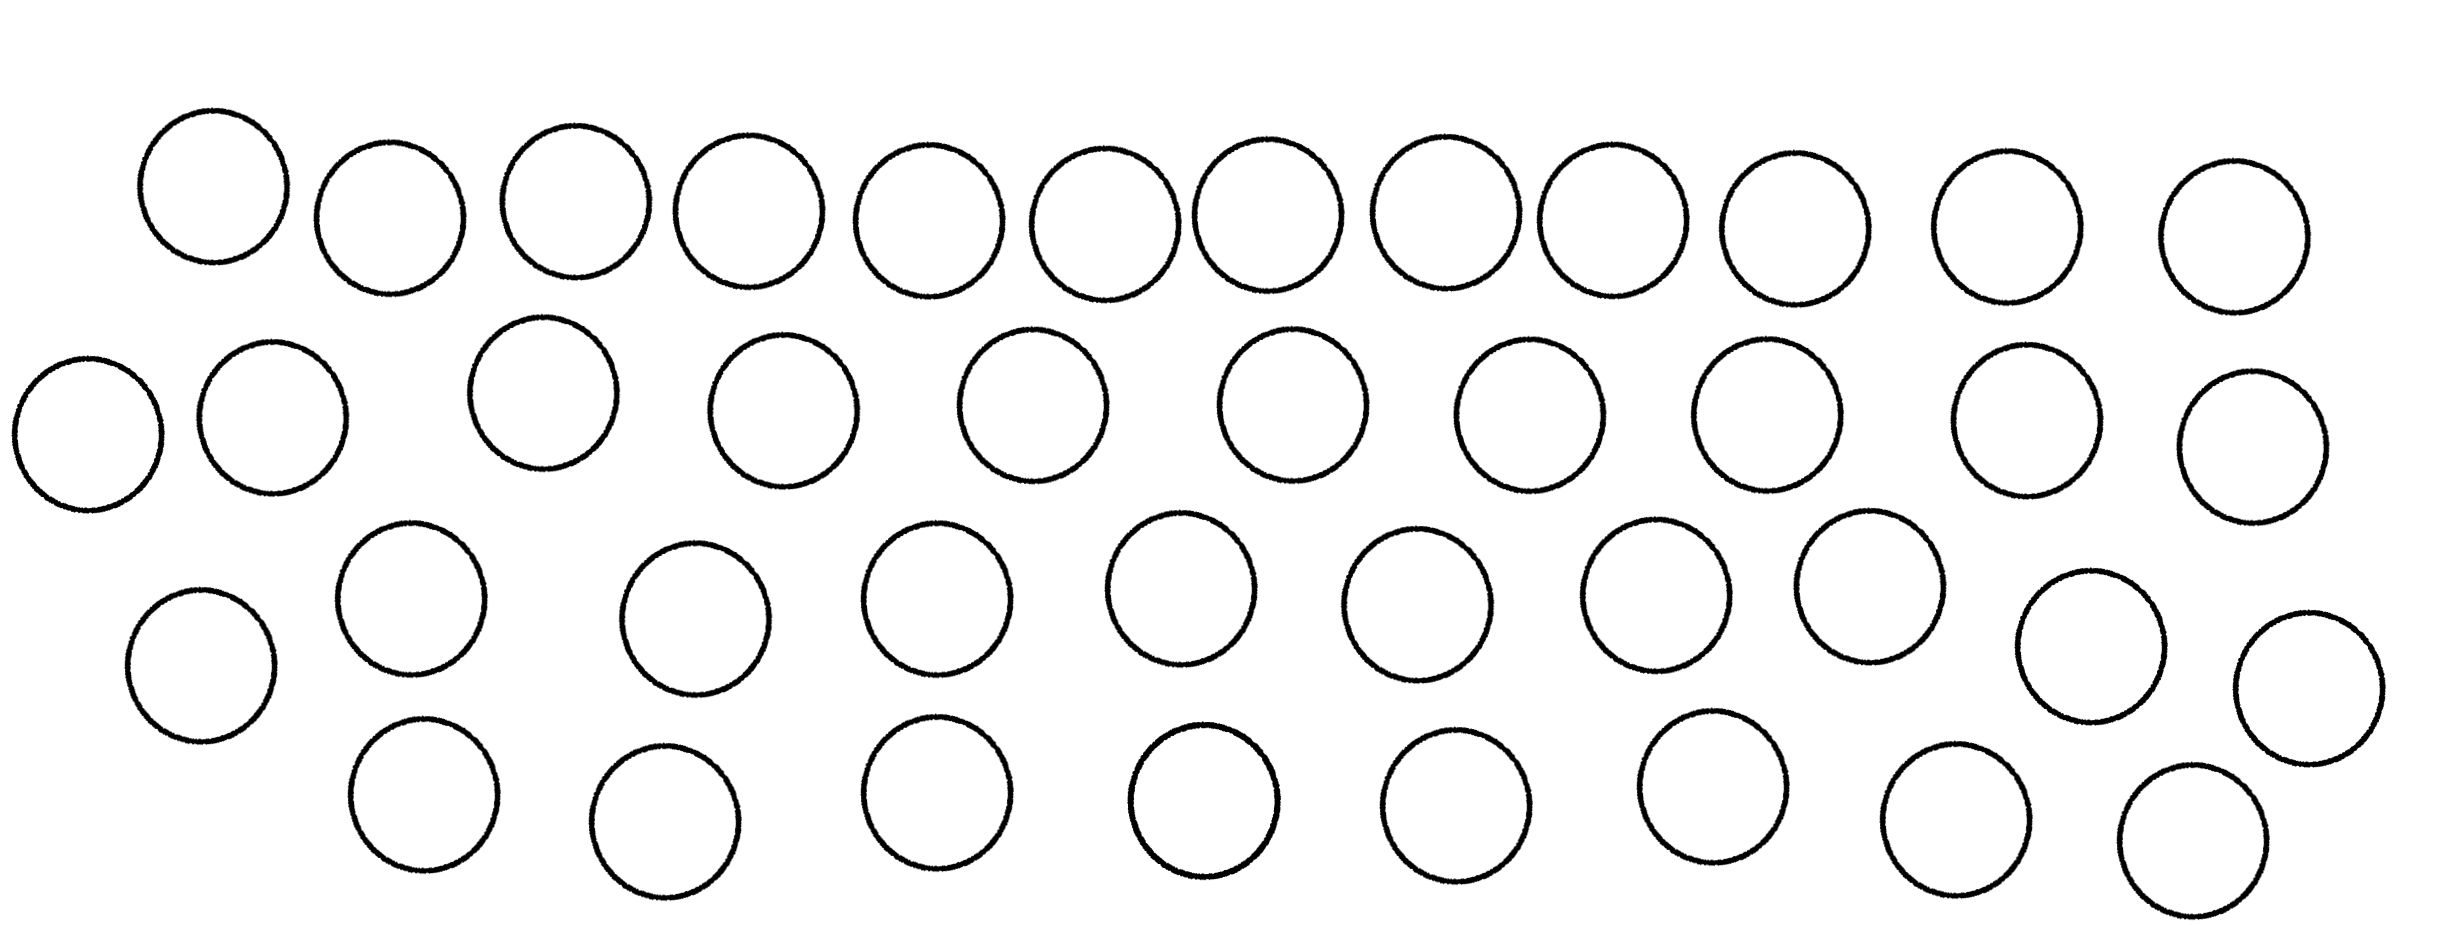
\includegraphics[height=1.7in]{images2/surfacet5.jpg}
\end{center}





 \end{frame}

%%%%%%%%%%%%%%%%%%%%%%%%%%%%%%%%%%%%%%%%%%%%%%%%%%%%%%%%%%%%%%%


\begin{frame}

\frametitle{Surface Tension and Capillarity}

Liquid surface $\leftrightarrow$ Stretched membrane under tension

  \begin{center}
  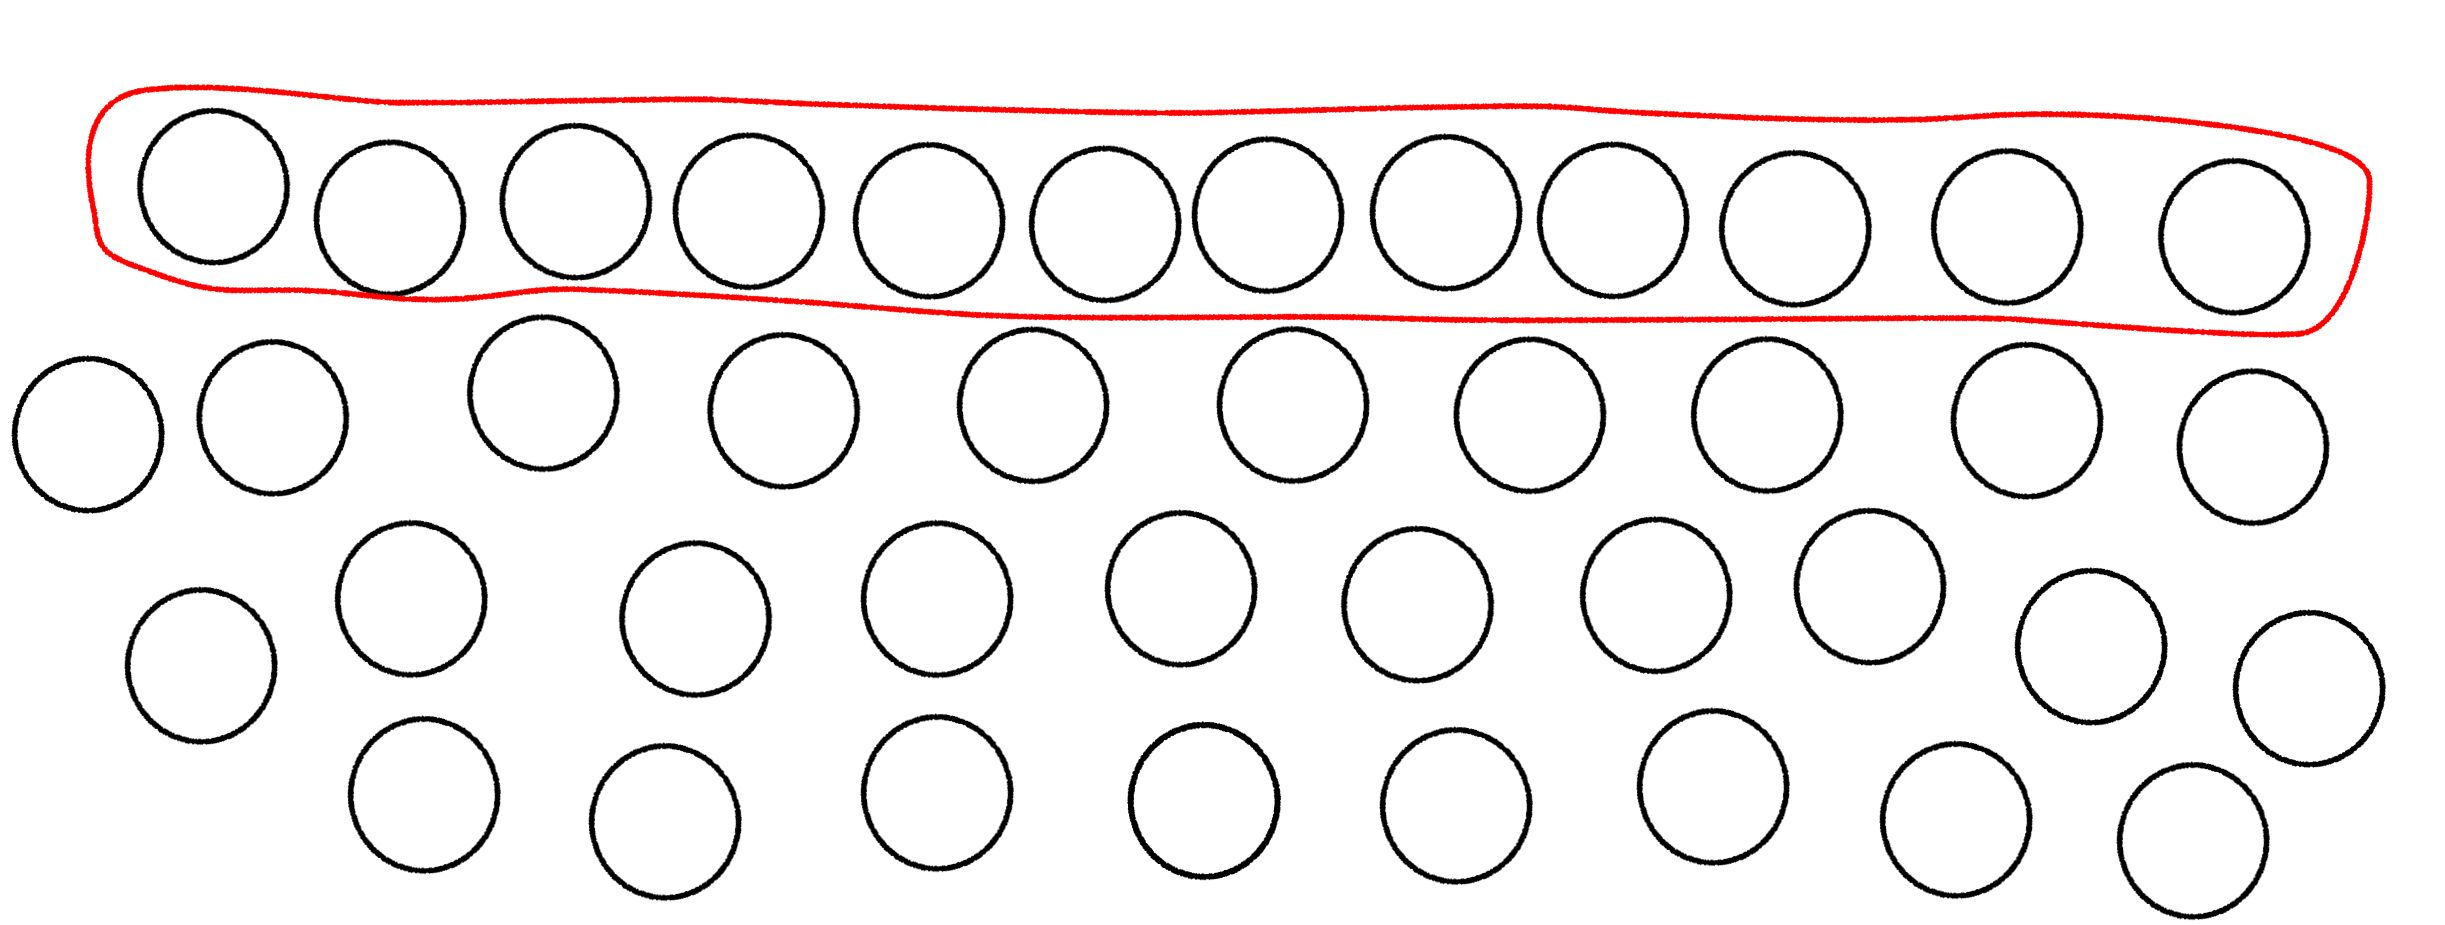
\includegraphics[height=1.7in]{images2/surfacet6.jpg}
\end{center}





 \end{frame}

%%%%%%%%%%%%%%%%%%%%%%%%%%%%%%%%%%%%%%%%%%%%%%%%%%%%%%%%%%%%%%%


\begin{frame}

\frametitle{Surface Tension and Capillarity}


Liquid not confined in a container.


  \begin{center}
  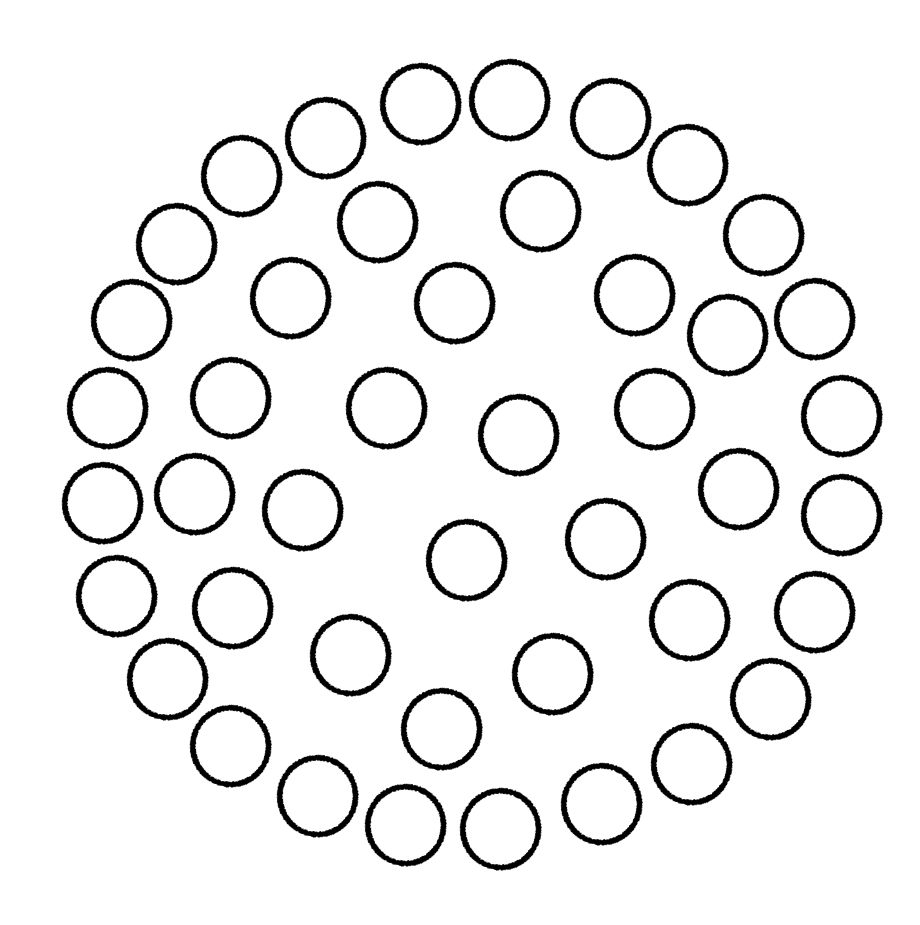
\includegraphics[height=1.7in]{images2/surfacet7.jpg}
\end{center}





 \end{frame}

%%%%%%%%%%%%%%%%%%%%%%%%%%%%%%%%%%%%%%%%%%%%%%%%%%%%%%%%%%%%%%%


\begin{frame}

\frametitle{Surface Tension and Capillarity}

Liquid not confined in a container.

  \begin{center}
  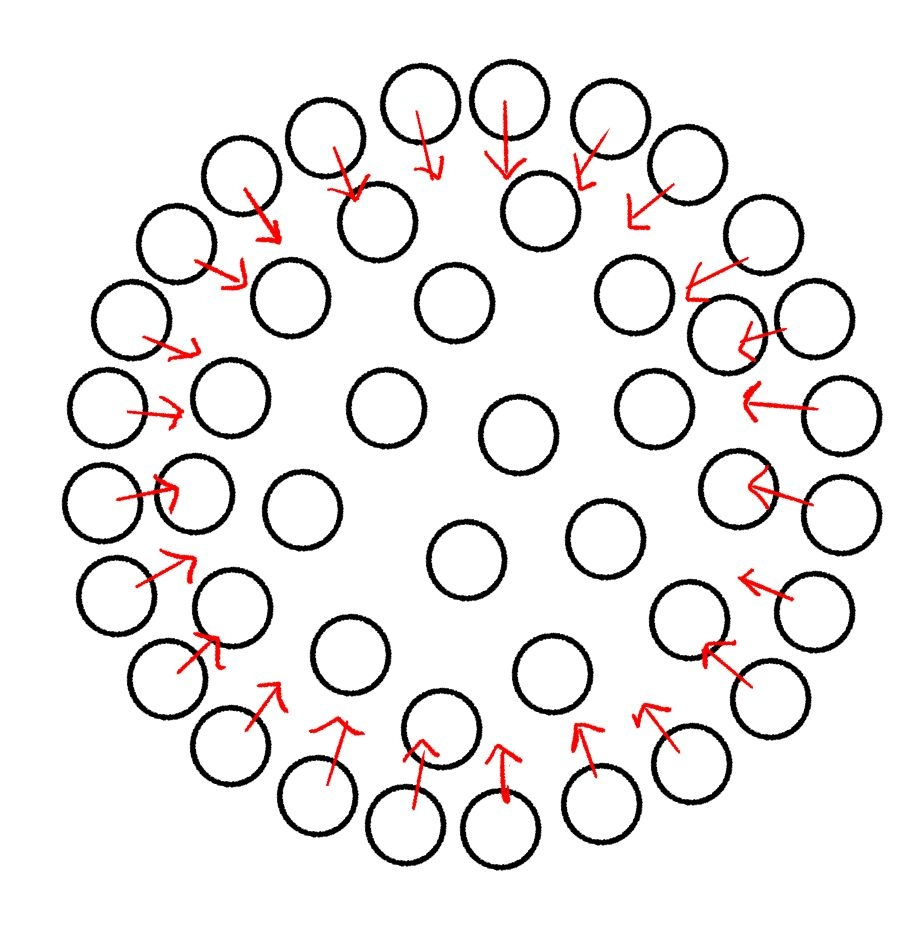
\includegraphics[height=1.7in]{images2/surfacet8.jpg}
\end{center}


\pause

 The ratio of surface area to volume is $4\pi r^2/(4\pi r^3/3)=3/r$


 \end{frame}

 %%%%%%%%%%%%%%%%%%%%%%%%%%%%%%%%%%%%%%%%%%%%%%%%%%%%%%%%%%%%%%%


\begin{frame}

  \frametitle{Surface Tension and Capillarity}


  


  
  

   \begin{columns}[c]
    \column{2in}  % slides are 3in high by 5in wide
 

    \begin{figure}[h!]
      \begin{center}
        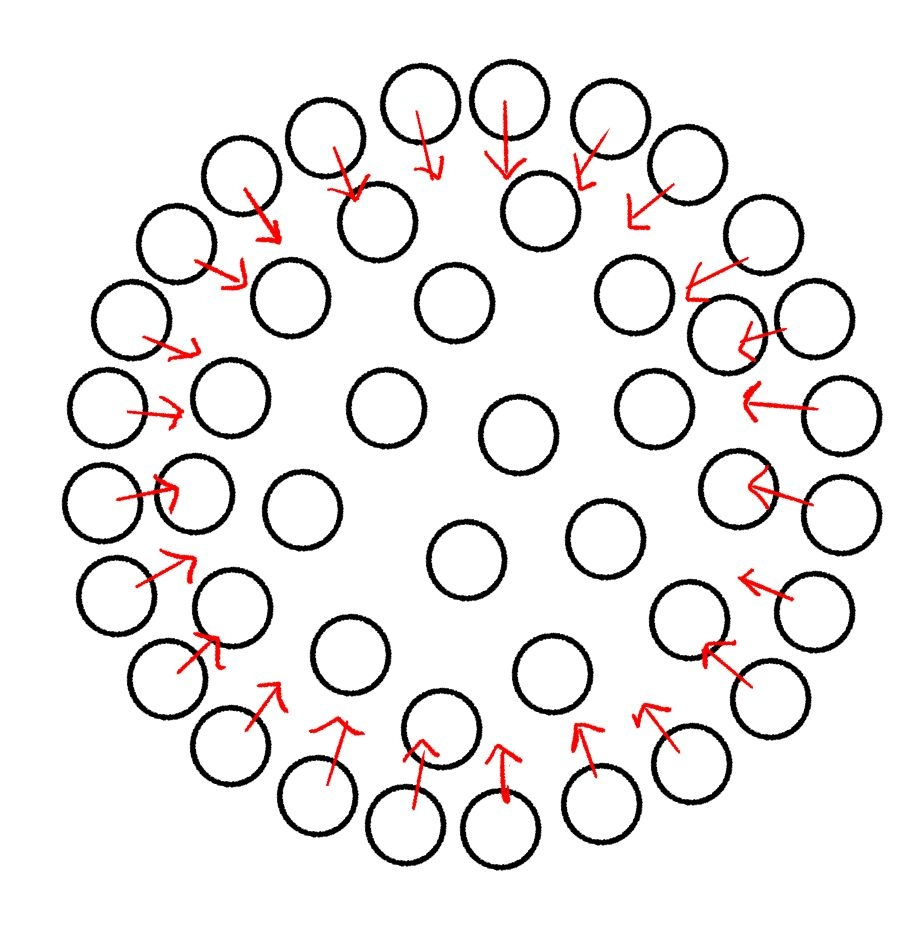
\includegraphics[height=1.6in]{images2/surfacet8.jpg}
      \end{center}
    \end{figure}

    
    \column{2.5in}
 
   \begin{itemize}
     \item  The ratio of surface area to volume is $4\pi r^2/(4\pi r^3/3)=3/r$ \pause
     \item  Large quantities of liquid $\rightarrow$  surface tension $<<$ pressure forces.\pause
     \item Small quantities of liquid $\rightarrow$  surface tension $>>$ pressure forces.
   \end{itemize}


    \end{columns}
 


   \end{frame}



%%%%%%%%%%%%%%%%%%%%%%%%%%%%%%%%%%%%%%%%%%%%%%%%%%%%%%%%%%%%%%%


\begin{frame}

\frametitle{Surface Tension and Capillarity}


\textcolor{mypink1}{How do we calculate the surface tension?}


\vspace{3mm}

\pause
\textbf{Surface Tension} (definition)

\vspace{3mm}

Force per unit length that acts perpendicular to any line or cut in a liquid surface, tending to pull the surface closed:

\vspace{3mm}
\pause

\begin{equation}
\boxed{\gamma=\frac{F}{\ell}}
\end{equation}



 \end{frame}





%%%%%%%%%%%%%%%%%%%%%%%%%%%%%%%%%%%%%%%%%%%%%%%%%%%%%%%%%%%%%%%


\begin{frame}

\frametitle{Surface Tension and Capillarity}






   \begin{columns}[c]
   \column{2in}  % slides are 3in high by 5in wide

    \begin{center}
  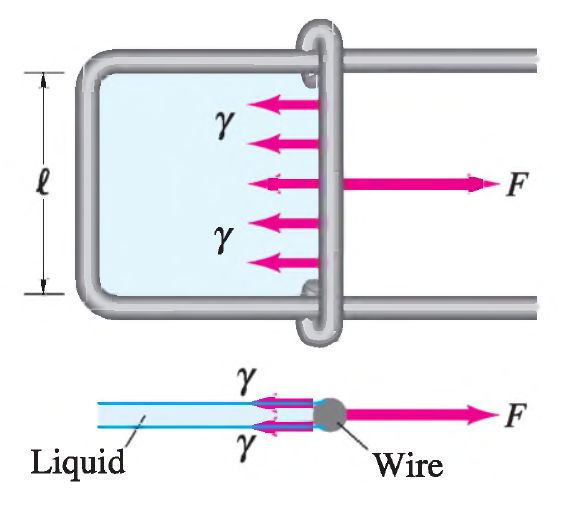
\includegraphics[height=1.7in]{images2/surfacet9.jpg}
\end{center}

\begin{equation*}
2 \gamma \ell=F \rightarrow \gamma=\boxed{\frac{F}{2\ell}}
\end{equation*}

   \column{2in}







    \begin{center}
  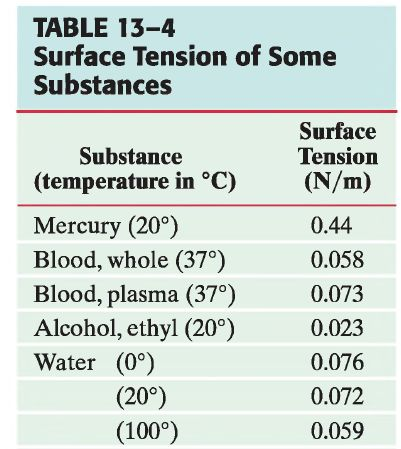
\includegraphics[height=2.2in]{images2/surfacet_table.jpg}
\end{center}

   \end{columns}



 \end{frame}

%%%%%%%%%%%%%%%%%%%%%%%%%%%%%%%%%%%%%%%%%%%%%%%%%%%%%%%%%%%%%%%
\stepcounter{examplef}

\begin{frame}

\frametitle{Example \theexamplef}



\textbf{Insect walks on water}. The base of an insect’s leg is approximately spherical in shape, with a radius of about
$2.0 \times 10^{-5} m$. The $0.0030~g$ mass of the insect is supported equally by its six legs.
Estimate the angle $\theta$ for an insect on the surface of water.
Assume the water temperature is 20°C.

    \begin{center}
  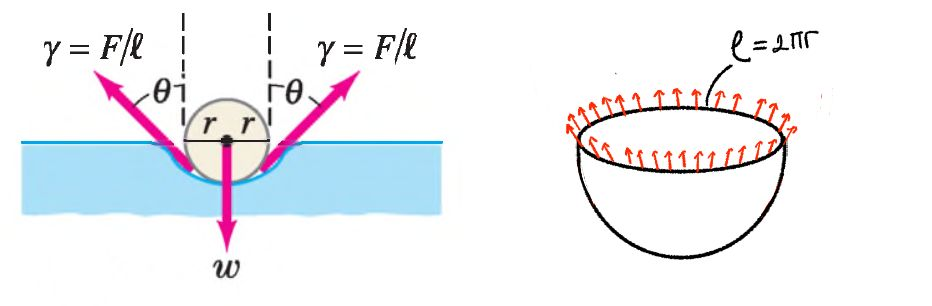
\includegraphics[height=1.5in]{images2/mosquito.jpg}
\end{center}


 \end{frame}

%%%%%%%%%%%%%%%%%%%%%%%%%%%%%%%%%%%%%%%%%%%%%%%%%%%%%%%%%%%%%%%


\begin{frame}

\frametitle{Surface Tension and Capillarity}


   \begin{columns}[c]
   \column{2in}  % slides are 3in high by 5in wide

      \begin{center}
  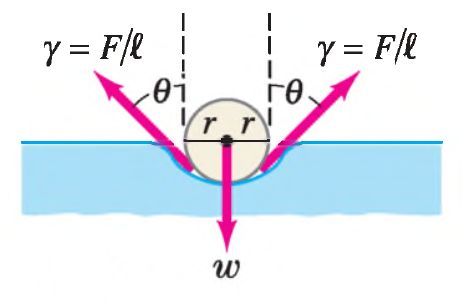
\includegraphics[height=1.5in]{images2/mosquito2.jpg}
\end{center}

   \column{2in}

\begin{equation*}
F\simeq(\gamma cos\theta) \ell=2\pi r \gamma cos\theta
\end{equation*}

\pause

\begin{equation*}
2\pi r \gamma cos\theta\simeq\frac{1}{6} mg
\end{equation*}

\pause

\begin{equation*}
\rightarrow cos \theta \simeq \frac{1}{6} \frac{mg}{2\pi r \gamma}
\end{equation*}

\pause

\begin{equation*}
\rightarrow cos \theta \simeq 0.54 \rightarrow \theta\simeq 57º
\end{equation*}

   \end{columns}




 \end{frame}


%%%%%%%%%%%%%%%%%%%%%%%%%%%%%%%%%%%%%%%%%%%%%%%%%%%%%%%%%%%%%%%




\begin{frame}

\frametitle{Surface Tension and Capillarity}



In tubes having very small diameters, liquids are observed to rise or fall relative
to the level of the surrounding liquid. This phenomenon is called capillarity

\vspace{3mm}



  \begin{center}
  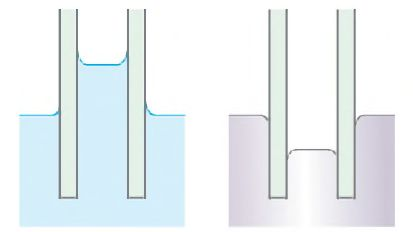
\includegraphics[height=1.7in]{images2/capillarity.jpg}
\end{center}




 \end{frame}

%%%%%%%%%%%%%%%%%%%%%%%%%%%%%%%%%%%%%%%%%%%%%%%%%%%%%%%%%%%%%%%


\begin{frame}

\frametitle{Surface Tension and Capillarity}


Whether a liquid wets a solid surface is determined by the relative strength of the
cohesive forces between the molecules of the liquid compared to the adhesive forces
between the molecules of the liquid and those of the container. Cohesion refers to the
force between molecules of the same type, whereas adhesion refers to the force between
molecules of different types.


  \begin{center}
  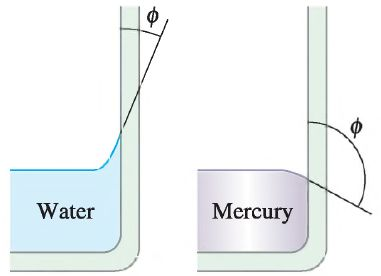
\includegraphics[height=1.5in]{images2/capillarity2.jpg}
\end{center}

 


 \end{frame}




%%%%%%%%%%%%%%%%%%%%%%%%%%%%%%%%%%%%%%%%%%%%%%%%%%%%%%%%%%%%%%%

\begin{frame}
  \frametitle{Fluids in motion}

We can distinguish two main types of fluid flow:
\vspace{3mm}

\begin{itemize}
\item Laminar Flow: Smooth flow $\rightarrow$ the neighbouring layers of the fluid slide by each other smoothly
\pause
\item Turbulent Flow: Above a certain speed, the flow is characterized by erratic, small, whirlpool-like circles called eddy currents or
eddies
\end{itemize}

\url{https://www.youtube.com/watch?v=WG-YCpAGgQQ}
  \end{frame}
  
%%%%%%%%%%%%%%%%%%%%%%%%%%%%%%%%%%%%%%%%%%%%%%%%%%%%%%%%%%%%%%%



\begin{frame}
\frametitle{Fluids in motion}

In streamline flow, each particle of the fluid follows
a smooth path, called a streamline, and these paths do not cross one another.
\vspace{3mm}

In a turbulent Flow, eddies absorb a great deal of energy, and although a certain
amount of internal friction called viscosity is present even during streamline flow,
it is much greater when the flow is turbulent.


\begin{center}
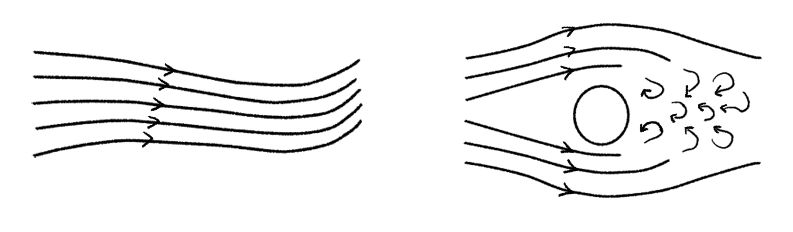
\includegraphics[height=1.3in]{images2/Fluids.jpg}
\end{center}

\end{frame}
%%%%%%%%%%%%%%%%%%%%%%%%%%%%%%%%%%%%%%%%%%%%%%%%%%%%%%%%%%%%%%%

\begin{frame}
 How do we know if the flow is laminar or turbulent?\pause $\rightarrow$ \textit{Reynold's number}
  \pause
  \vspace{3mm}
  
  The equations that describe the motion of the elements of fluids are:

  \begin{equation*}
    \boxed{\rho \vec{a}=-\nabla P-\rho \nabla \phi +\vec{f}_{vis}} ~~~Navier~ Stokes~eq.
    \end{equation*}

  \end{frame}

%%%%%%%%%%%%%%%%%%%%%%%%%%%%%%%%%%%%%%%%%%%%%%%%%%%%%%%%%%%%%%%

  

%%%%%%%%%%%%%%%%%%%%%%%%%%%%%%%%%%%%%%%%%%%%%%%%%%%%%%%%%%%%%%%

  
\begin{frame}
  We can write an equivalent dimensionless equation, so we can get rid of the units:
   
     \begin{equation*}
    \frac{d\vec{v'}}{dt'}=-\nabla' P' -\nabla' \phi' +\frac{1}{\mathsf{R}_e} \nabla'^2 \vec{v'}
       \end{equation*}
   \pause
   \begin{equation*}
  \boxed{\mathsf{R}_e=\frac{\rho v D}{\eta}}
       \end{equation*}
  \pause
  \vspace{2mm}
  
  $v:caracteristic~velocity$
  
  $D:caracteristic~dimension$
  
   $\rho:caracteristic~density$
  
     \end{frame}

   %%%%%%%%%%%%%%%%%%%%%%%%%%%%%%%%%%%%%%%%%%%%%%%%%%%%%%%%%%%%%%%

  
\begin{frame}
  We can write an equivalent dimensionless equation, so we can get rid of the units:
   
     \begin{equation*}
      \underbrace{ \frac{d\vec{v'}}{dt'}}_{\textcolor{mypink1}{acceleration}}=      \underbrace{-\nabla' P'}_{\textcolor{mypink1}{pressure}} -\underbrace{-\nabla' \phi'}_{\textcolor{mypink1}{gravity}}+ \overbrace{\frac{1}{\mathsf{R}_e} \nabla'^2 \vec{v'}}^{\textcolor{mypink1}{viscosity}}
       \end{equation*}

\vspace{5mm}
\pause

\textcolor{mypink1}{Now we can compare acceleration with pressure and gravity.}
  
     \end{frame}

          
%%%%%%%%%%%%%%%%%%%%%%%%%%%%%%%%%%%%%%%%%%%%%%%%%%%%%%%%%%%%%%%


  



  
   \begin{frame}
$\mathsf{R}_e>>1 $    

   
     \begin{equation*}
      \mbox{\fontsize{20}{20}\selectfont\( \frac{d\vec{v'}}{dt'}
      \)} = \mbox{\fontsize{20}{20}\selectfont\(-\nabla' P' -\nabla' \phi' \)} + \mbox{\fontsize{10}{10}\selectfont\( \frac{1}{\mathsf{R}_e} \nabla'^2 \vec{v'} \)}
       \end{equation*}
       \pause

       \vspace{5mm}
   
   \textcolor{mypink1}{Viscosity is not important}

       \end{frame}
  
       
  %%%%%%%%%%%%%%%%%%%%%%%%%%%%%%%%%%%%%%%%%%%%%%%%%%%%%%%%%%%%%%%

\begin{frame}
    $\mathsf{R}_e<<1 $    
    
       
         \begin{equation*}
          \mbox{\fontsize{10}{10}\selectfont\( \mathsf{R}_e\frac{d\vec{v'}}{dt'}
          \)} = \mbox{\fontsize{20}{20}\selectfont\(-\frac{1}{\eta}\nabla P -\frac{\rho}{\eta}\nabla \phi \)} + \mbox{\fontsize{20}{20}\selectfont\(  \nabla'^2 \vec{v'} \)}
           \end{equation*}
      
    \pause

    \vspace{5mm}

\textcolor{mypink1}{We no longer have time in our equation!!!}

\pause

\vspace{2mm}

\textcolor{mypink1}{You can go forward in time and then do the same thing backward in time and  "undo" the process.}

\end{frame}

     
%%%%%%%%%%%%%%%%%%%%%%%%%%%%%%%%%%%%%%%%%%%%%%%%%%%%%%%%%%%%%%%

\subsection{Generalization}
\begin{frame}

\frametitle{Generalization}


To fully describe a fluid, we need the velocity vector field, that is  $\vec{v}(x,y,z,t)$.

  \begin{center}
  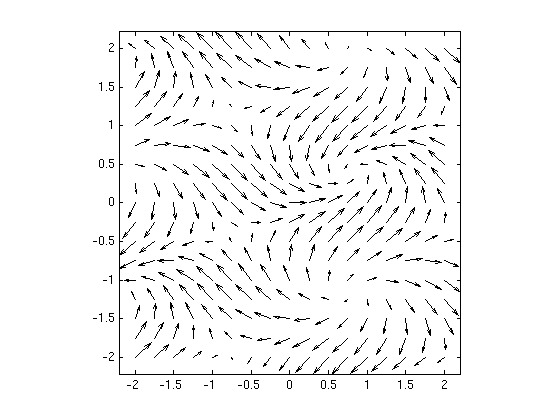
\includegraphics[height=2.in]{images2/vectorial.png}
\end{center}


$\rightarrow$ \url{https://www.youtube.com/watch?v=VJ2ZDLQk3IQ} 

 \end{frame}


%%%%%%%%%%%%%%%%%%%%%%%%%%%%%%%%%%%%%%%%%%%%%%%%%%%%%%%%%%%%%%%

\begin{frame}

\frametitle{Generalization}


   \begin{columns}[c]
   \column{1.7in}  % slides are 3in high by 5in wide

Which are the equations that describe the velocity field?
\pause

    \begin{center}
  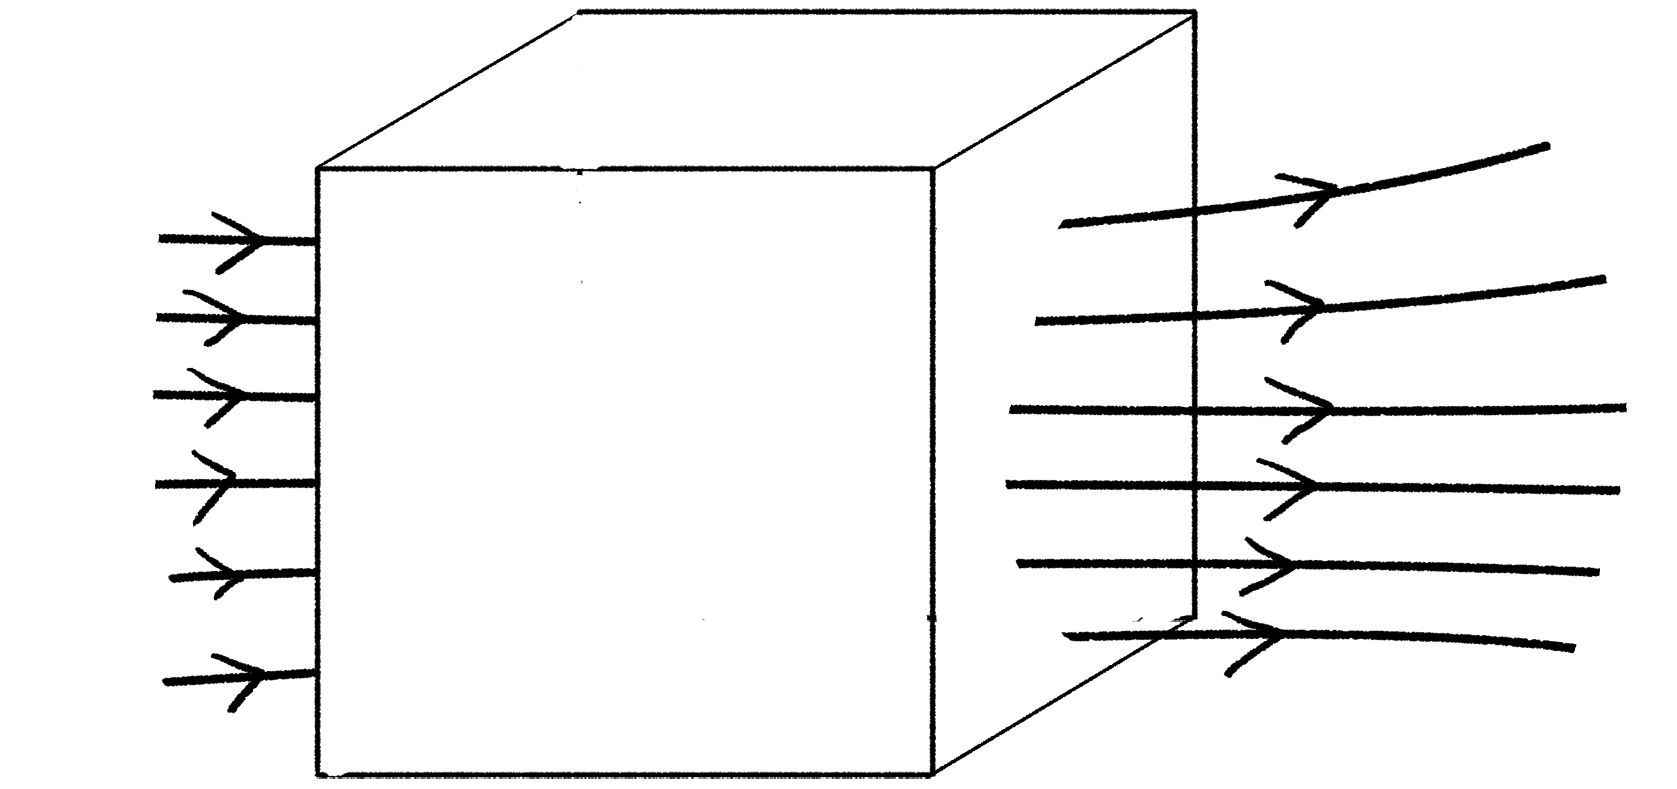
\includegraphics[height=0.8in]{images2/generalization2.jpg}
\end{center}

   \column{2.3in}

\pause

The mass flow rate  passing $A_{X1}$ is

\begin{equation*}
\rho v_xdydz
\end{equation*}

\pause
The mass flow rate  passing $A_{x2}$ is


\begin{equation*}
\rho  (v_x+\frac{\partial v_x}{\partial x} dx)dydz
\end{equation*}

\pause
The difference between the mass flow rate entering through $A_{X2}$ and $A_{X1}$ is,

\begin{equation*}
\rho \frac{\partial v_x}{\partial x} dydzdx
\end{equation*}

\end{columns}







 \end{frame}




%%%%%%%%%%%%%%%%%%%%%%%%%%%%%%%%%%%%%%%%%%%%%%%%%%%%%%%%%%%%%%%

\begin{frame}

\frametitle{Generalization}

If we do the same for $y$ and $z$,

\begin{equation*}
\rho \frac{\partial v_y}{\partial y} dydzdx
\end{equation*}

\begin{equation*}
\rho \frac{\partial v_z}{\partial z} dydzdx
\end{equation*}


Then, the difference between the total flow entering and exiting the volume is

\begin{equation*}
\rho( \frac{\partial v_x}{\partial x}+ \frac{\partial v_y}{\partial y}+ \frac{\partial v_z}{\partial z} )dydzdx
\end{equation*}


 \end{frame}

%%%%%%%%%%%%%%%%%%%%%%%%%%%%%%%%%%%%%%%%%%%%%%%%%%%%%%%%%%%%%%%



\begin{frame}

\frametitle{Generalization}

If the entering flux is equatl to the exiting flux


 \begin{equation*}
\rho( \frac{\partial v_x}{\partial x}+ \frac{\partial v_y}{\partial y}+ \frac{\partial v_z}{\partial z} )dydzdx=0
\end{equation*}
\pause

Then,

 \begin{equation*}
( \frac{\partial v_x}{\partial x}+ \frac{\partial v_y}{\partial y}+ \frac{\partial v_z}{\partial z} )=0
\end{equation*}

\pause

or using the nabla operator,


 \begin{equation*}
\nabla \cdot \vec{v}=0
\end{equation*}

 \end{frame}





%%%%%%%%%%%%%%%%%%%%%%%%%%%%%%%%%%%%%%%%%%%%%%%%%%%%%%%%%%%%%%%


\begin{frame}

\frametitle{Generalization}

If the density is not constant, 


 \begin{equation*}
\nabla \cdot (\rho \vec{v})=0
\end{equation*}

If the entering flux is not equal to exiting flux,

 \begin{equation*}
\nabla \cdot (\rho \vec{v})=-\frac{\partial \rho}{\partial t}
\end{equation*}

This is the Hydrodynamic Equation of Continuity.
 \end{frame}





%%%%%%%%%%%%%%%%%%%%%%%%%%%%%%%%%%%%%%%%%%%%%%%%%%%%%%%%%%%%%%%



\begin{frame}

\frametitle{Generalization}
Then we have one equation for 3 unknowns.

\pause

\vspace{3mm}

 We will get our next equation from Newton’s law which tells us how the
velocity changes because of the forces:


 \begin{equation*}
\rho \vec{a}=-\nabla P-\rho \nabla \phi +\vec{f}_{vis}
\end{equation*}

\pause

\vspace{3mm}
We  suppose that the liquid is “thin” the viscosity is unimportant, so we will omit $f_{vis}\rightarrow$ \textit{Dry Water Flow} 

 \end{frame}



%%%%%%%%%%%%%%%%%%%%%%%%%%%%%%%%%%%%%%%%%%%%%%%%%%%%%%%%%%%%%%%



\begin{frame}

What is the acceleration?
\vspace{3mm}
\pause



\begin{equation*}
IT~IS~NOT~\vec{a}=\frac{\partial \vec{v}}{\partial t}!!!!
\end{equation*}
\vspace{3mm}

\pause
To obtain the acceleration we must calculate,
\vspace{3mm}

\begin{equation*}
\frac{\Delta \vec{v}}{\Delta t}
\end{equation*}


for an actual displacement of an element of fluid. That is,


\begin{equation*}
\frac{\Delta \vec{v}}{\Delta t}=v_x \frac{\partial \vec{v}}{\partial x}+v_y \frac{\partial \vec{v}}{\partial y}+v_z \frac{\partial \vec{v}}{\partial z}+\frac{\partial \vec{v}}{\partial t}
\end{equation*}



 \end{frame}




%%%%%%%%%%%%%%%%%%%%%%%%%%%%%%%%%%%%%%%%%%%%%%%%%%%%%%%%%%%%%%%

\begin{frame}

Using the nabla,


\begin{equation*}
\vec{a}=(\vec{v}\cdot \nabla)\vec{v}+\frac{\partial \vec{v}}{\partial t}
\end{equation*}
\pause
Then, the second Newton's Law takes the form,

 \begin{equation*}
(\vec{v}\cdot \nabla)\vec{v}+\frac{\partial \vec{v}}{\partial t}=-\frac{\nabla P}{\rho}- \nabla \phi 
\end{equation*}
\pause
This equation can be expressed as,

 \begin{equation*}
\Omega\times\vec{v}+\frac{1}{2}\nabla v^2+\frac{\partial \vec{v}}{\partial t}=-\frac{\nabla P}{\rho}- \nabla \phi 
\end{equation*}

\pause
where,


 \begin{equation*}
\Omega=\nabla\times\vec{v}
\end{equation*}
\pause
Is the curl of $\vec{v}$ and is called vorticity.


 \end{frame}


%%%%%%%%%%%%%%%%%%%%%%%%%%%%%%%%%%%%%%%%%%%%%%%%%%%%%%%%%%%%%%%


\begin{frame}

\textbf{Physical interpretation of the curl}
\vspace{3mm}

\pause
The curl is the micro-circulation per unit area of $ \vec{v}$ and  has the same direction than the normal to the surface

\pause

 \begin{equation*}
\nabla\times\vec{v}=\left(\lim_{\Delta S\to 0}\frac{1}{\Delta S} \oint_S \vec{v}\cdot d\vec{r}\right)\cdot\hat{n}
\end{equation*}
\vspace{3mm}


\pause
If you put a little piece of dirt—not an infinitesimal point—at any place in the liquid it will rotate with the angular velocity $\Omega/2$.
\vspace{3mm}


\pause

$\rightarrow$ \url{https://mathinsight.org/curl_ idea} 


 \end{frame}

%%%%%%%%%%%%%%%%%%%%%%%%%%%%%%%%%%%%%%%%%%%%%%%%%%%%%%%%%%%%%%%






%%%%%%%%%%%%%%%%%%%%%%%%%%%%%%%%%%%%%%%%%%%%%%%%%%%%%%%%%%%%%%%
 \end{document}
%%%%%%%%%%%%%%%%%%%%%%%%%%%%%%%%%%%%%%%%%%%%%%%%%%%%%%%%%%%%%%%